% =============================================================================
%  SIMULACIÓN DE SISTEMAS - TP4
%  Grupo 05 - Sebastián Caules, Jerónimo Esquivel, Andrés Cortese
%  Dinámica Molecular regida por el paso temporal
%  Sistema 1: oscilador amortiguado (solo resultados, consigna)
%  Sistema 2: recinto circular con obstáculo fijo (estructura completa)
%
%  Versión ORAL (animaciones embebidas con \movie del paquete multimedia).
%  Compilar y proyectar con pympress para autoplay.
%  Estructura según Guía de Presentaciones de la cátedra (secciones explícitas
%  Introducción / Implementación / Simulaciones / Resultados / Conclusiones).
% =============================================================================

\documentclass[10pt,aspectratio=169]{beamer}
\usetheme{Warsaw}
\usecolortheme{default}
\setbeamertemplate{navigation symbols}{}

% Header: miniframes con puntos de progreso por sección, sin subsection
\useoutertheme[subsection=false,footline=empty]{miniframes}

% Footer: solo número de diapositiva a la derecha (Guía 1.2)
\setbeamertemplate{footline}{%
    \hfill{\footnotesize\insertframenumber\,/\,\inserttotalframenumber}\hspace{8pt}\vspace{4pt}%
}

\setbeamercolor{frametitle}{bg=blue!70!black, fg=white}

% --- Paquetes ---
\usepackage[utf8]{inputenc}
\usepackage[T1]{fontenc}
\usepackage[spanish]{babel}
\usepackage{amsmath,amssymb,amsfonts}
\usepackage{bm}
\usepackage{graphicx}
\usepackage{siunitx}
\usepackage{xcolor}
\usepackage{tikz}
\usetikzlibrary{arrows.meta,positioning,shapes.geometric,calc}
\usepackage{multimedia}

% --- Macros ---
% \simvideo{poster sin ext}{video sin ext}
\newlength{\vidW}
\newlength{\vidH}
\newcommand{\simvideo}[2]{%
  \setlength{\vidH}{0.62\textheight}%
  \setlength{\vidW}{\vidH}%
  \movie[autostart,loop,width=\vidW,height=\vidH,poster]{%
    \includegraphics[width=\vidW,height=\vidH]{#1.png}%
  }{#2.mp4}%
}

% Placeholder para figuras / animaciones faltantes (no rompe compilación).
\newcommand{\missingfig}[2]{%
  \begin{tikzpicture}
    \draw[thick,dashed,red!55!black] (0,0) rectangle (0.92\linewidth,0.62\textheight);
    \node[align=center,red!55!black,text width=0.86\linewidth]
      at (0.46\linewidth,0.31\textheight)
      {\textbf{Falta:} #1\\[6pt]\footnotesize\itshape #2};
  \end{tikzpicture}%
}
\newcommand{\figorplaceholder}[3]{%
  \IfFileExists{#1.png}{\includegraphics[#2]{#1}}{%
    \missingfig{{\ttfamily\detokenize{#1.png}}}{#3}%
  }%
}
\newcommand{\videoorplaceholder}[3]{%
  \IfFileExists{#1.png}{\simvideo{#1}{#2}}{%
    \missingfig{{\ttfamily\detokenize{#1.png}}\,/\,{\ttfamily\detokenize{#2.mp4}}}{#3}%
  }%
}

% Vectores en negrita sin itálica (Guía 3.5)
\newcommand{\vect}[1]{\mathbf{#1}}

% Cita en la esquina inferior izquierda
\newcommand{\framecite}[1]{%
  \begin{tikzpicture}[remember picture,overlay]
    \node[anchor=south west,font=\tiny,text=black!60]
      at ([xshift=6pt,yshift=4pt]current page.south west) {#1};
  \end{tikzpicture}}

% Slide separadora de sub-sección dentro del Sistema 2 (sin marcar como
% \section para no agregar puntos al header de miniframes; cumple 1.13).
\newcommand{\sectiondivider}[1]{%
  \begin{frame}[plain,c]
    \centering
    {\usebeamercolor[fg]{structure}\fontsize{42}{50}\selectfont #1\par}
  \end{frame}%
}

% --- Metadatos ---
\title[TP4 -- DM paso temporal]{Dinámica Molecular regida por el paso temporal}
\subtitle{Trabajo Práctico N\textsuperscript{o} 4}
\author[Caules, Esquivel, Cortese]{Sebastián Caules \and Jerónimo Esquivel \and Andrés Cortese}
\institute[ITBA]{Instituto Tecnológico de Buenos Aires \\ 72.25 -- Simulación de Sistemas -- Grupo 05}
\date{18 de mayo de 2026}

\begin{document}

% =============================================================================
% PORTADA
% =============================================================================
{
    \setbeamertemplate{headline}{}
    \setbeamertemplate{footline}{}
    \begin{frame}[plain]
        \titlepage
    \end{frame}
}

% =============================================================================
% SISTEMA 1 -- solo resultados, ~2 slides, < 1 min, ANTES de Sistema 2
% (consigna: sin introducción / sin integradores / sin animaciones / sin conclusiones)
% =============================================================================
\section{Sistema 1}

\begin{frame}{Trayectorias $r(t)$ -- numérica vs.\ analítica}
    \centering
    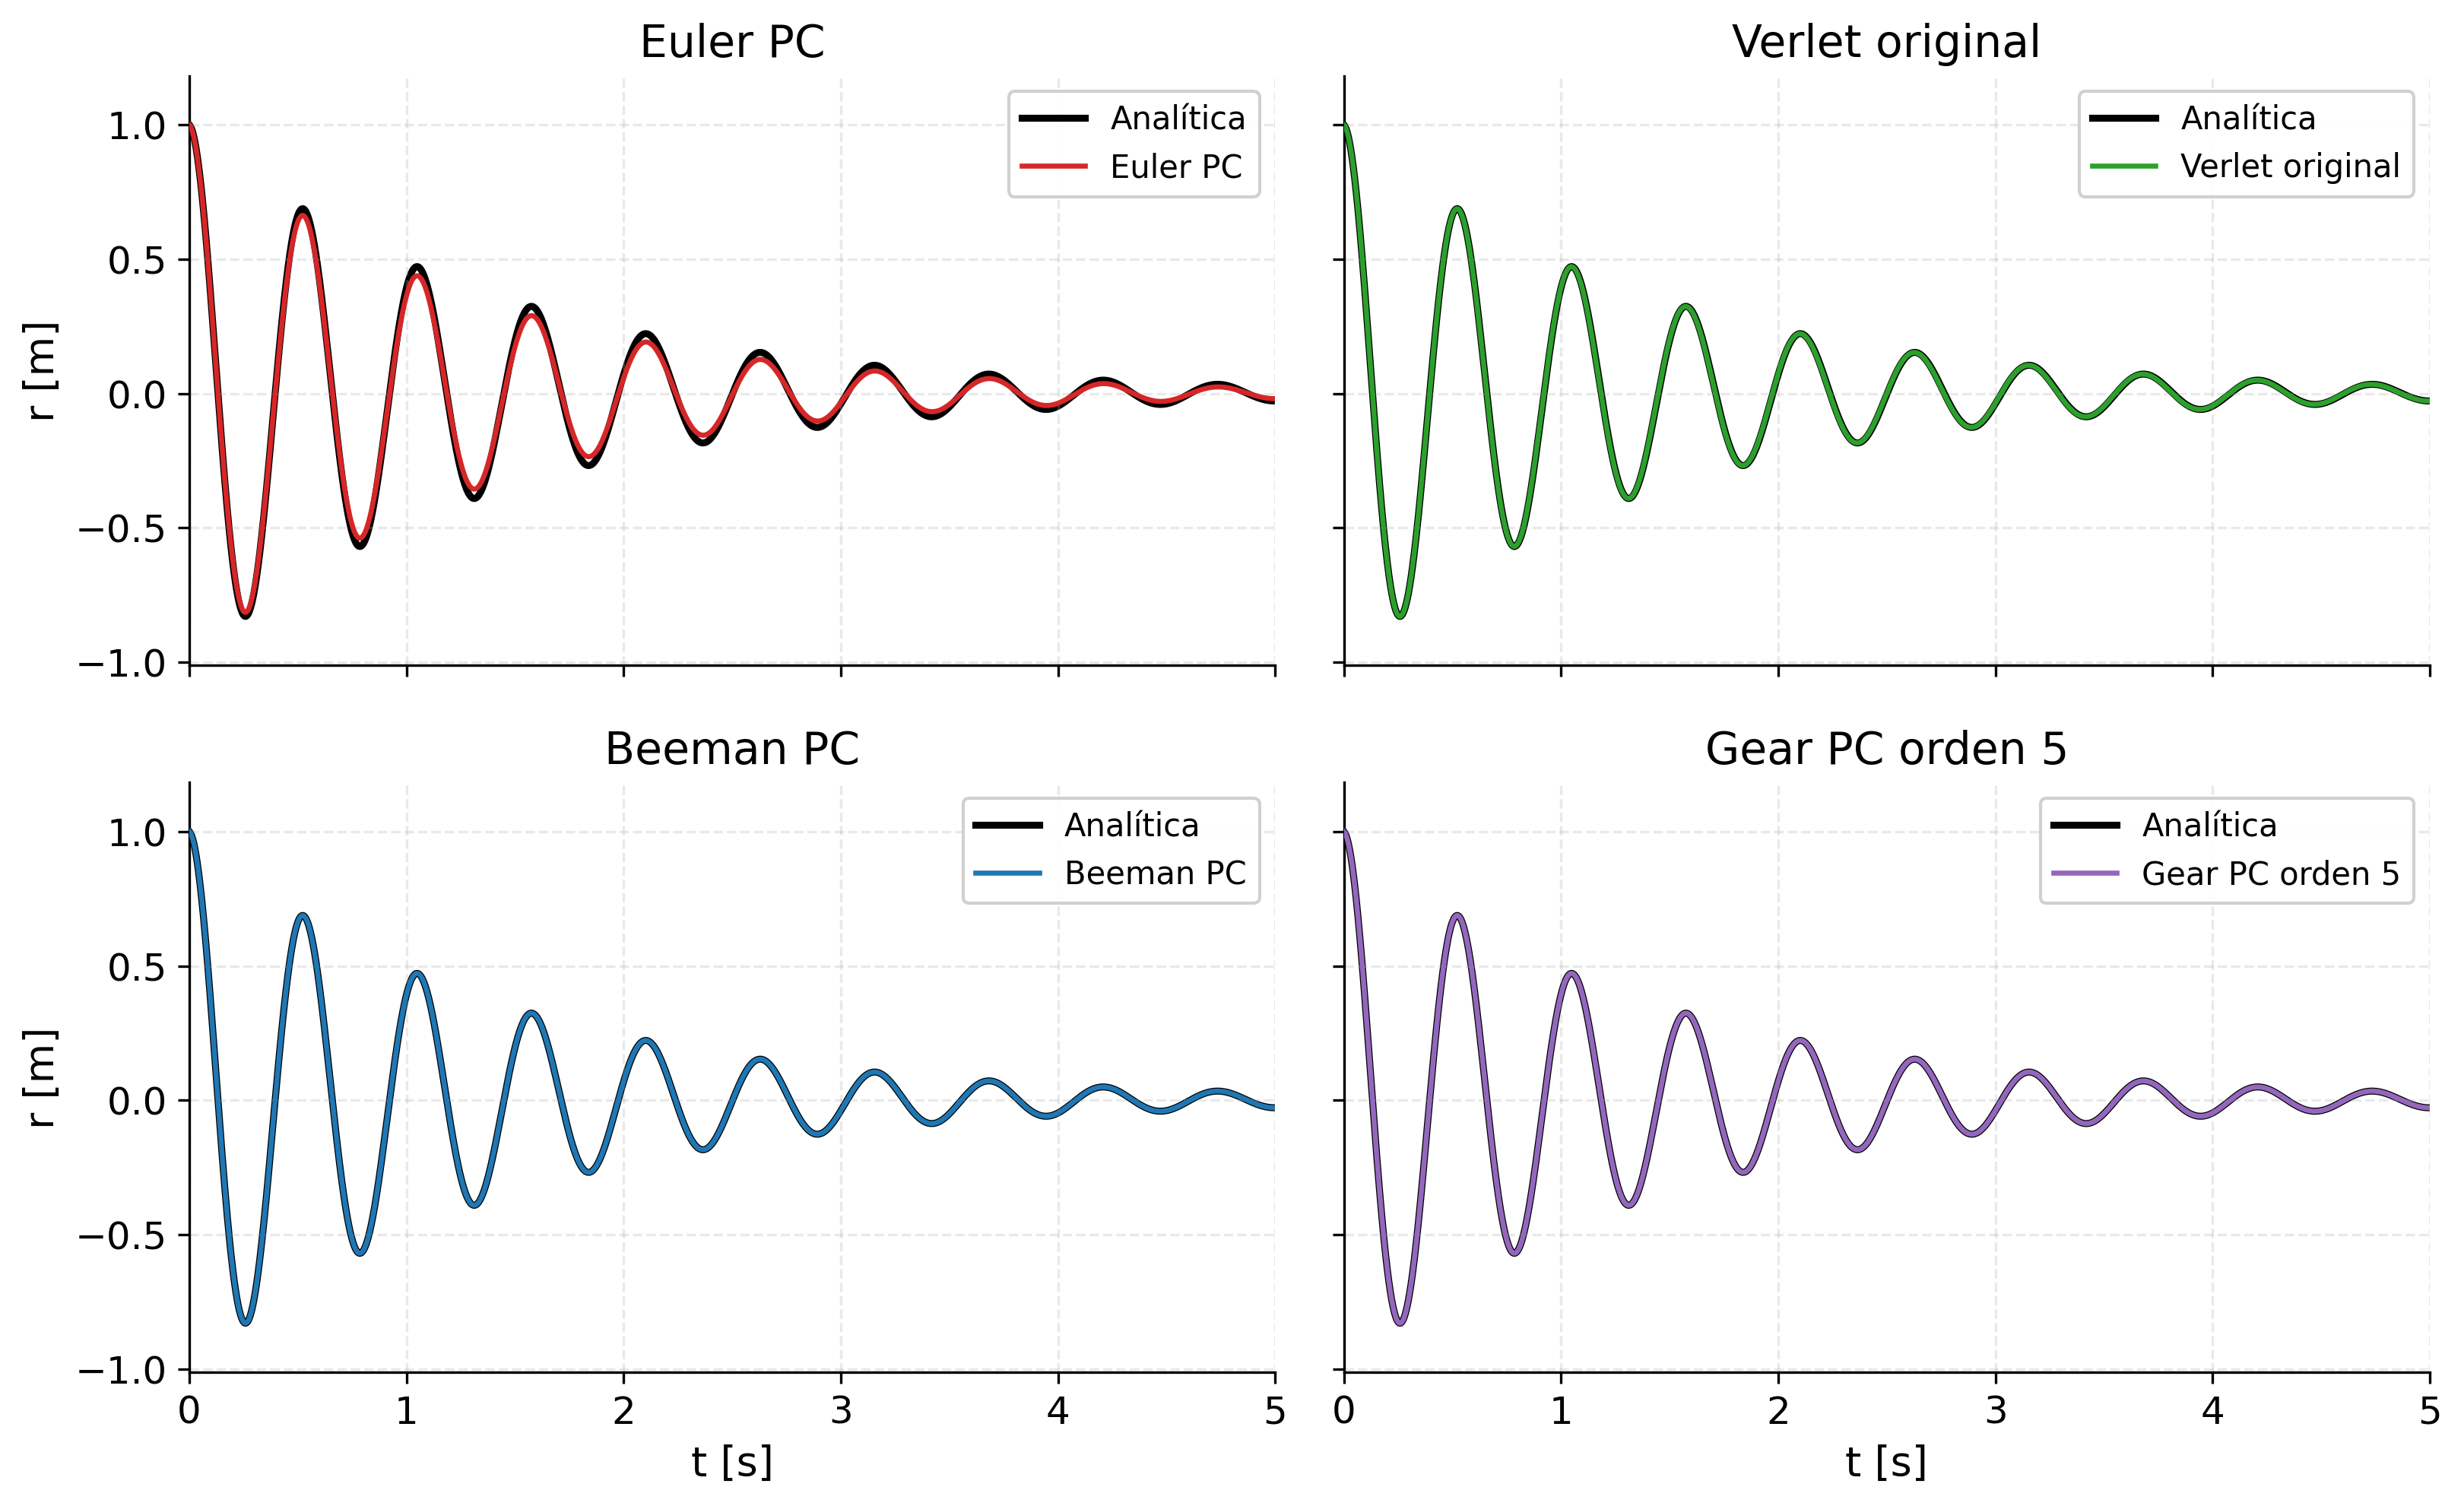
\includegraphics[width=0.95\linewidth,height=0.78\textheight,keepaspectratio]{figures/01_s1_r_vs_t.png}

    \vspace{0.1cm}
    {\footnotesize $m=70$ kg, $k=10^4$ N/m, $\gamma=100$ kg/s, $r(0)=1$ m, $v(0)=-A\gamma/(2m)$, $\Delta t=10^{-3}$ s, $t_f=5$ s}
\end{frame}

\begin{frame}{Error cuadrático medio vs.\ $\Delta t$}
    \centering
    
\includegraphics[width=0.85\linewidth,height=0.82\textheight,keepaspectratio]{figures/02_s1_ecm_vs_dt.png}
\end{frame}

% =============================================================================
% SISTEMA 2 -- estructura completa según la Guía
% =============================================================================
\section{Sistema 2}

\begin{frame}[plain,c]
    \centering
    {\usebeamercolor[fg]{structure}\fontsize{42}{50}\selectfont Sistema 2\par}
    \vspace{0.5cm}
    {\large Recinto circular con obstáculo fijo}\par
    {\large DM regida por paso temporal con fuerza elástica blanda}
\end{frame}

% --- Introducción ------------------------------------------------------------
\sectiondivider{Introducción}

\begin{frame}{Sistema real y motivación}
        \begin{itemize}
            \item Sistemas físicos modelables como partículas con interacciones por colisión: gases diluidos, granos, partículas brownianas.
            \item Sistema real simulado: glóblulos blancos del sistema inmunológico
        \end{itemize}
    \end{frame}

\begin{frame}{Modelo matemático}
    \begin{columns}[T]
        \begin{column}{0.95\textwidth}
            \textbf{Ecuaciones de movimiento (Newton)}
            \[
                m_i\,\ddot{\vect{r}}_i \;=\; \vect{F}_i^{\,Tot} \;=\; \sum_{j \neq i} \vect{F}_{ij}
            \]

            \vspace{0.4em}
            \textbf{Interacción de a pares (elástica, de corto alcance)}
            \[
                \vect{F}_{ij} =
                \begin{cases}
                    k\,\xi_{ij}\,\vect{e}_{ij} & \text{si } \xi_{ij} > 0 \\[2pt]
                    \vect{0} & \text{si } \xi_{ij} \leq 0
                \end{cases}
            \]

            \vspace{0.2em}
            con la superposición y el versor normal definidos como
            \[
                \xi_{ij} = (r_i + r_j) - |\vect{x}_i - \vect{x}_j|,
                \qquad
                \vect{e}_{ij} = \frac{\vect{x}_i - \vect{x}_j}{|\vect{x}_i - \vect{x}_j|}.
            \]

            \vspace{0.3em}
            \footnotesize
            La fuerza actúa únicamente durante el contacto ($\xi_{ij} > 0$),
            es decir, los choques tienen duración finita y se resuelven a lo largo
            de varios pasos temporales.
        \end{column}
    \end{columns}
\end{frame}

% --- Implementación ----------------------------------------------------------
\sectiondivider{Implementación}

\begin{frame}{Arquitectura del proyecto}
    \centering
    \begin{tikzpicture}[
        font=\footnotesize,
        node distance=4mm and 5mm,
        every node/.style={align=center, rounded corners=2pt, inner sep=3pt},
        entry/.style ={draw, fill=blue!12,   minimum width=22mm, minimum height=7mm},
        sim/.style   ={draw, fill=blue!25,   minimum width=28mm, minimum height=8mm},
        mod/.style   ={draw, fill=gray!12,   minimum width=28mm, minimum height=6.5mm},
        csvbox/.style={draw, fill=orange!18, minimum width=28mm, minimum height=7mm},
        post/.style  ={draw, dashed, fill=gray!06, minimum width=28mm, minimum height=7mm},
        flow/.style  ={-{Latex[length=1.6mm]}, semithick, gray!70!black},
    ]
        % --- Sistema 1 (izquierda) ---
        \node[entry] (m1) {\textbf{\texttt{Main1}}\\\scriptsize ECM($\Delta t$)};
        \node[sim, below=of m1] (s1) {\texttt{sim/Simulator}\\\scriptsize oscilador 1D};
        \node[mod, below=of s1] (i1) {\texttt{integrators/}\\\scriptsize Euler -- Verlet -- Beeman -- Gear-5};

        % --- Sistema 2 (derecha) ---
        \node[entry, right=22mm of m1] (m2) {\textbf{\texttt{Main2}}\\\scriptsize \texttt{-{}-experiment}};
        \node[mod, below=8mm of m2, fill=blue!06, minimum width=58mm] (exp)
            {\texttt{experiments/}: \texttt{energy\_dt\_scan} $\cdot$ \texttt{timing} $\cdot$ \texttt{jvsn} $\cdot$ \texttt{ksweep}};
        \node[sim, below=of exp] (s2) {\texttt{sim/Simulator2D}\\\scriptsize loop $\Delta t$ con \emph{hook} por paso};
        \node[mod, below left=4mm and -10mm of s2] (i2) {\texttt{integrators/}\\\scriptsize Velocity-Verlet $\cdot$ Beeman};
        \node[mod, below=of s2] (ph) {\texttt{physics/}\\\scriptsize \texttt{ForceModel} $\cdot$ \texttt{CellIndexMethod}};
        \node[mod, below right=4mm and -10mm of s2] (ob) {\texttt{observables/}\\\scriptsize \texttt{CfcTracker} $\cdot$ perfiles radiales};

        % --- Salida + postproceso ---
        \node[csvbox, below=18mm of ph] (csv) {CSV (\texttt{results/})};
        \node[post, right=8mm of csv] (plot) {\texttt{plotter/} (Python)\\\scriptsize no entregable};

        % --- Flechas ---
        \draw[flow] (m1) -- (s1);
        \draw[flow] (s1) -- (i1);
        \draw[flow] (m2) -- (exp);
        \draw[flow] (exp) -- (s2);
        \draw[flow] (s2) -- (i2);
        \draw[flow] (s2) -- (ph);
        \draw[flow] (s2) -- (ob);
        \draw[flow] (i1.south) |- ($(csv.west)+(-4mm,0)$) -- (csv.west);
        \draw[flow] (ph) -- (csv);
        \draw[flow] (csv) -- (plot);

        % --- Etiquetas de columna ---
        \node[above=1mm of m1, font=\scriptsize\bfseries, text=blue!50!black] {Sistema 1};
        \node[above=1mm of m2, font=\scriptsize\bfseries, text=blue!50!black] {Sistema 2};
    \end{tikzpicture}
\end{frame}

\begin{frame}{Motor de simulación}
    \begin{enumerate}\setlength\itemsep{3pt}
        \item Sembrar $N$ partículas por rejection sampling: posiciones sin
              solapamiento, $|\vect{v}| = v_0$ con ángulo uniforme en $[0, 2\pi)$.
        \item Indexar en \emph{Cell Index Method} (celda $= 2\,r_{\max}$):
              vecinos en $\mathcal{O}(1)$ por partícula.
        \item \textbf{Mientras} $t < t_f$:
        \begin{enumerate}\setlength\itemsep{1pt}
            \item Calcular fuerzas: pares en contacto ($\xi>0$),
                  obstáculo, borde. \hfill $\mathcal{O}(N)$
            \item Integrar un paso $\Delta t$ con Velocity-Verlet 2D.
                  \hfill $\mathcal{O}(N)$
            \item Detectar flancos de contacto y actualizar el estado
                  fresca\,/\,usada de cada partícula.
            \item Acumular $C_{fc}(t)$ con resolución $\Delta t$;
                  muestrear estado cada $\Delta t_2$ para los perfiles
                  radiales.
        \end{enumerate}
    \end{enumerate}
    \vspace{0.2cm}
    \textbf{Integrador}: Velocity-Verlet 2D (simpléctico, $\vect{F} = \vect{F}(\vect{x})$).
\end{frame}

\begin{frame}{Integradores implementados}
    \begin{columns}[T]
        \column{0.50\textwidth}
        \textbf{Sistema 1} -- $\vect{F}(r,\dot r)$ con dependencia en $\dot r$
        \begin{itemize}\setlength\itemsep{2pt}
            \item Euler predictor-corrector
            \item Verlet original
            \item Beeman predictor-corrector
            \item Gear PC orden 5 \quad ($\alpha_0 = 3/16$)
        \end{itemize}
        \vspace{0.15cm}
        {\footnotesize Inicialización analítica de las derivadas superiores en Gear-5 (diferenciando $\ddot r = -(k/m)r - (\gamma/m)\dot r$).}
        \column{0.50\textwidth}
        \textbf{Sistema 2} -- $\vect{F}(\vect{x})$ (sólo posiciones)
        \begin{itemize}\setlength\itemsep{2pt}
            \item \textbf{Velocity-Verlet 2D} (default, simpléctico)
            \item Beeman 2D (verificación cruzada)
        \end{itemize}
        \vspace{0.15cm}
        \textbf{Vecinos}: \emph{Cell Index Method} con celda $= 2\,r_{\max}$ (un paso de fuerzas en $\mathcal{O}(N)$).
    \end{columns}
\end{frame}

% --- Simulaciones ------------------------------------------------------------
\sectiondivider{Simulaciones}

\begin{frame}{Sistema particular}
    \begin{columns}[T]
        \begin{column}{0.55\textwidth}
            \begin{itemize}\setlength\itemsep{2pt}
                \item Recinto circular de diámetro $L = \SI{80}{m}$.
                \item Obstáculo fijo central, radio $r_0 = \SI{1}{m}$.
                \item $N$ partículas; $r = \SI{1}{m}$, $m = \SI{1}{kg}$.
                \item $|\vect{v}_0| = \SI{1}{m/s}$, dirección uniforme $\in [0,2\pi)$.
                \item Distribución inicial uniforme, sin solapamiento.
                \item Estados:
                \begin{itemize}
                    \item \textcolor{green!55!black}{\textbf{Fresca}}: al tocar el obstáculo $\rightarrow$ usada.
                    \item \textcolor{violet!70!black}{\textbf{Usada}}: al tocar el borde $\rightarrow$ fresca.
                \end{itemize}
            \end{itemize}
        \end{column}
        \begin{column}{0.45\textwidth}
            \centering
            \begin{tikzpicture}[scale=0.85]
                \draw[thick] (0,0) circle (3);
                \fill[violet!70!black] (0,0) circle (0.25);
                \foreach \x/\y in {1.2/0.5, -1.5/0.8, 0.3/-1.8, 1.8/-1.2, -0.9/-2.1, -2.0/-0.4, 0.7/2.1, 1.9/1.5}
                \fill[green!60!black] (\x,\y) circle (0.12);
                \foreach \x/\y in {-0.5/1.6, 2.2/0.3, -1.8/1.8}
                \fill[violet!70!black] (\x,\y) circle (0.12);
                \draw[<->] (-3,-3.4) -- (3,-3.4) node[midway,below,font=\small]{$L$};
                \node[font=\scriptsize,anchor=west] at (0.32,0.0) {$r_0$};
            \end{tikzpicture}
        \end{column}
    \end{columns}
\end{frame}

\begin{frame}{Parámetros y realizaciones}
    \begin{columns}[T]
        \begin{column}{0.50\textwidth}
            \textbf{Parámetros variables}
            \begin{itemize}\setlength\itemsep{2pt}
                \item $N \in [100, 1000]$ con pasos de $100$.
                \item $k \in \{10^1, 10^5\}$ \si{N/m}.
                \item $k_{\text{ref}} = 10^3$ \si{N/m}.
            \end{itemize}
            \vspace{0.2cm}
            \textbf{Parámetros fijos}
            \begin{itemize}\setlength\itemsep{2pt}
                \item $t_f = \SI{500}{s}$.
                \item $\Delta t_2 = \SI{0.05}{s}$.
            \end{itemize}
        \end{column}
        \begin{column}{0.50\textwidth}
            \textbf{Realizaciones}
            \begin{itemize}\setlength\itemsep{2pt}
                \item (1.1) Una realización por N.
                \item (1.2, 1.3) $M = 100$ realizaciones por N con $k_{\text{ref}}$ fijo.
                \item (1.4) $M=100$ para $k \leq 10^3$ y $M=30$ para $k > 10^3$.
            \end{itemize}
        \end{column}
    \end{columns}
\end{frame}

\begin{frame}{Observables (1/2) -- scanning rate}
    \textbf{Cambio de estado:} con $C_{fc}(t)$ el contador acumulado de
    transiciones fresca$\to$usada en $[0, t]$,
    \[
        C_{fc}(t) = \sum_{n=1}^{\lfloor t/\Delta t\rfloor}
                    \#\{\text{transiciones fresca}\to\text{usada en el paso } n\}.
    \]
    Sólo se cuenta el \textbf{primer $\Delta t$} de cada contacto con el obstáculo.

    \vspace{0.3cm}
    \textbf{Scanning rate} $J$: pendiente de $C_{fc}(t)$ en la ventana de régimen
    estacionario. Calculado por ajuste lineal.
\end{frame}

\begin{frame}{Observables (2/2) -- perfiles radiales}
    Capas concéntricas de ancho $\mathrm{d}S = \SI{0.2}{m}$; en cada snapshot,
    $P_f^{\,\text{in}}(S, t)$: partículas \emph{frescas} con velocidad radial
    entrante, $\vect{x}_j\!\cdot\!\vect{v}_j < 0$, en la capa $S$.
    $n_k^{\,\text{in}}(S, t) = |P_f^{\,\text{in}}(S,t)|$ en la realización $k$.
    \[
        \langle\rho_f^{\,\text{in}}\rangle(S)
          = \frac{1}{M\,T}\sum_{k=1}^{M}\sum_{t}\frac{n_k^{\,\text{in}}(S,t)}{A(S)},
        \qquad
        A(S) = 2\pi S\,\mathrm{d}S
    \]
    \[
        |\langle v_f^{\,\text{in}}\rangle(S)|
          = \left|\frac{1}{M\,T'}\!\!
                  \sum_{\substack{k,t\\ n_k^{\,\text{in}}>0}}
                  \frac{1}{n_k^{\,\text{in}}}
                  \!\!\sum_{j\in P_f^{\,\text{in}}}\!\!\tfrac{\vect{x}_j\!\cdot\!\vect{v}_j}{|\vect{x}_j|}\right|,
        \qquad
        J^{\,\text{in}}(S) = \langle\rho_f^{\,\text{in}}\rangle(S)\,
                             |\langle v_f^{\,\text{in}}\rangle(S)|
    \]
    {\footnotesize $T$: snapshots promediados ($t_f/\Delta t_2 = 10^4$). \quad
                   $T'$: subconjunto de snapshots con $n_k^{\,\text{in}}(S,t) > 0$
                   (los snapshots con capa vacía se omiten del promedio de $v$).}
\end{frame}

% =============================================================================
% RESULTADOS
% =============================================================================
\section{Resultados}

\begin{frame}[plain,c]
    \centering
    {\usebeamercolor[fg]{structure}\fontsize{48}{56}\selectfont Resultados\par}
\end{frame}

% =============================================================================
% ANIMACIONES variando N (k = 10^3 fijo)
% =============================================================================
\begin{frame}{Animación -- $N = 100$, $k = 10^{3}$ \si{N/m}}
    \begin{columns}[T]
        \begin{column}{0.68\textwidth}
            \centering
            \simvideo{figures/N=100}{videos/N=100}
        \end{column}
        \begin{column}{0.32\textwidth}
            \textbf{Condiciones}
            \begin{itemize}
                \item $N = 100$
                \item $k = 10^{3}$ \si{N/m}
                \item $\Delta t = \SI{e-3}{s}$
            \end{itemize}
        \end{column}
    \end{columns}
\end{frame}

\begin{frame}{Animación -- $N = 1000$, $k = 10^{3}$ \si{N/m}}
    \begin{columns}[T]
        \begin{column}{0.68\textwidth}
            \centering
            \simvideo{figures/N=1000}{videos/N=1000}
        \end{column}
        \begin{column}{0.32\textwidth}
            \textbf{Condiciones}
            \begin{itemize}
                \item $N = 1000$
                \item $k = 10^{3}$ \si{N/m}
                \item $\Delta t = \SI{e-3}{s}$
            \end{itemize}
        \end{column}
    \end{columns}
\end{frame}

% =============================================================================
% Validación de Δt @ k=10³: evolución de E(t) y pendiente Se
% =============================================================================
\begin{frame}{Conservación de energía vs.\ $\Delta t$ -- $k = 10^{3}$ \si{N/m}}
    \begin{columns}[T]
        \begin{column}{0.68\textwidth}
            \centering
            
\includegraphics[width=\linewidth,height=0.70\textheight,keepaspectratio]{figures/03d_s2_energy_dt_scan_k1e3.png}
        \end{column}
        \begin{column}{0.32\textwidth}
            \textbf{Métrica}\\[2pt]
            \resizebox{\linewidth}{!}{$\dfrac{\Delta E_{\text{tot}}(t)}{E_0} = \dfrac{E_{\text{tot}}(t)-E_0}{E_0}$}
            \vspace{0.2cm}

            \textbf{Observación}
            \begin{itemize}\setlength\itemsep{1pt}
                \item Curva por $\Delta t$, gradiente viridis.
                \item Umbral de deriva: $\pm 1\%$.
                \item $\Delta t$ chico $\Rightarrow$ deriva acotada.
            \end{itemize}
            \vspace{0.1cm}
            \textbf{Parámetros}: $N = 800$, $t_f = \SI{2000}{s}$.
        \end{column}
    \end{columns}
\end{frame}

\begin{frame}{Pendiente $S_e$ del error de energía y $\Delta t$ elegido -- $k = 10^{3}$}
    \begin{columns}[T]
        \begin{column}{0.68\textwidth}
            \centering
            
\includegraphics[width=\linewidth,height=0.70\textheight,keepaspectratio]{figures/03f_s2_energy_dt_slope_k1e3.png}
        \end{column}
        \begin{column}{0.32\textwidth}
            \textbf{$S_e$}\\[2pt]
            Pendiente lineal de
            $\Delta E_{\text{tot}}/E_0$ vs.\ $t$ (regresión).
            \vspace{0.15cm}

            \textbf{Criterio}
            \begin{itemize}\setlength\itemsep{1pt}
                \item $|S_e|$ chico $\Rightarrow$ drift acotado.
                \item Bajar $\Delta t$ baja $|S_e|$ hasta el piso numérico.
            \end{itemize}
            \vspace{0.1cm}
            \textbf{$\Delta t$ elegido} para $k = 10^{3}$:
            $\Delta t = \SI{2.0e-3}{s}$
\end{column}
    \end{columns}
\end{frame}

% =============================================================================
% 1.1 Tiempo de ejecución -- comparación con TP3
% =============================================================================
\begin{frame}{Tiempo de ejecución vs.\ $N$ -- comparación con TP3}
    \begin{columns}[T]
        \begin{column}{0.68\textwidth}
            \centering
            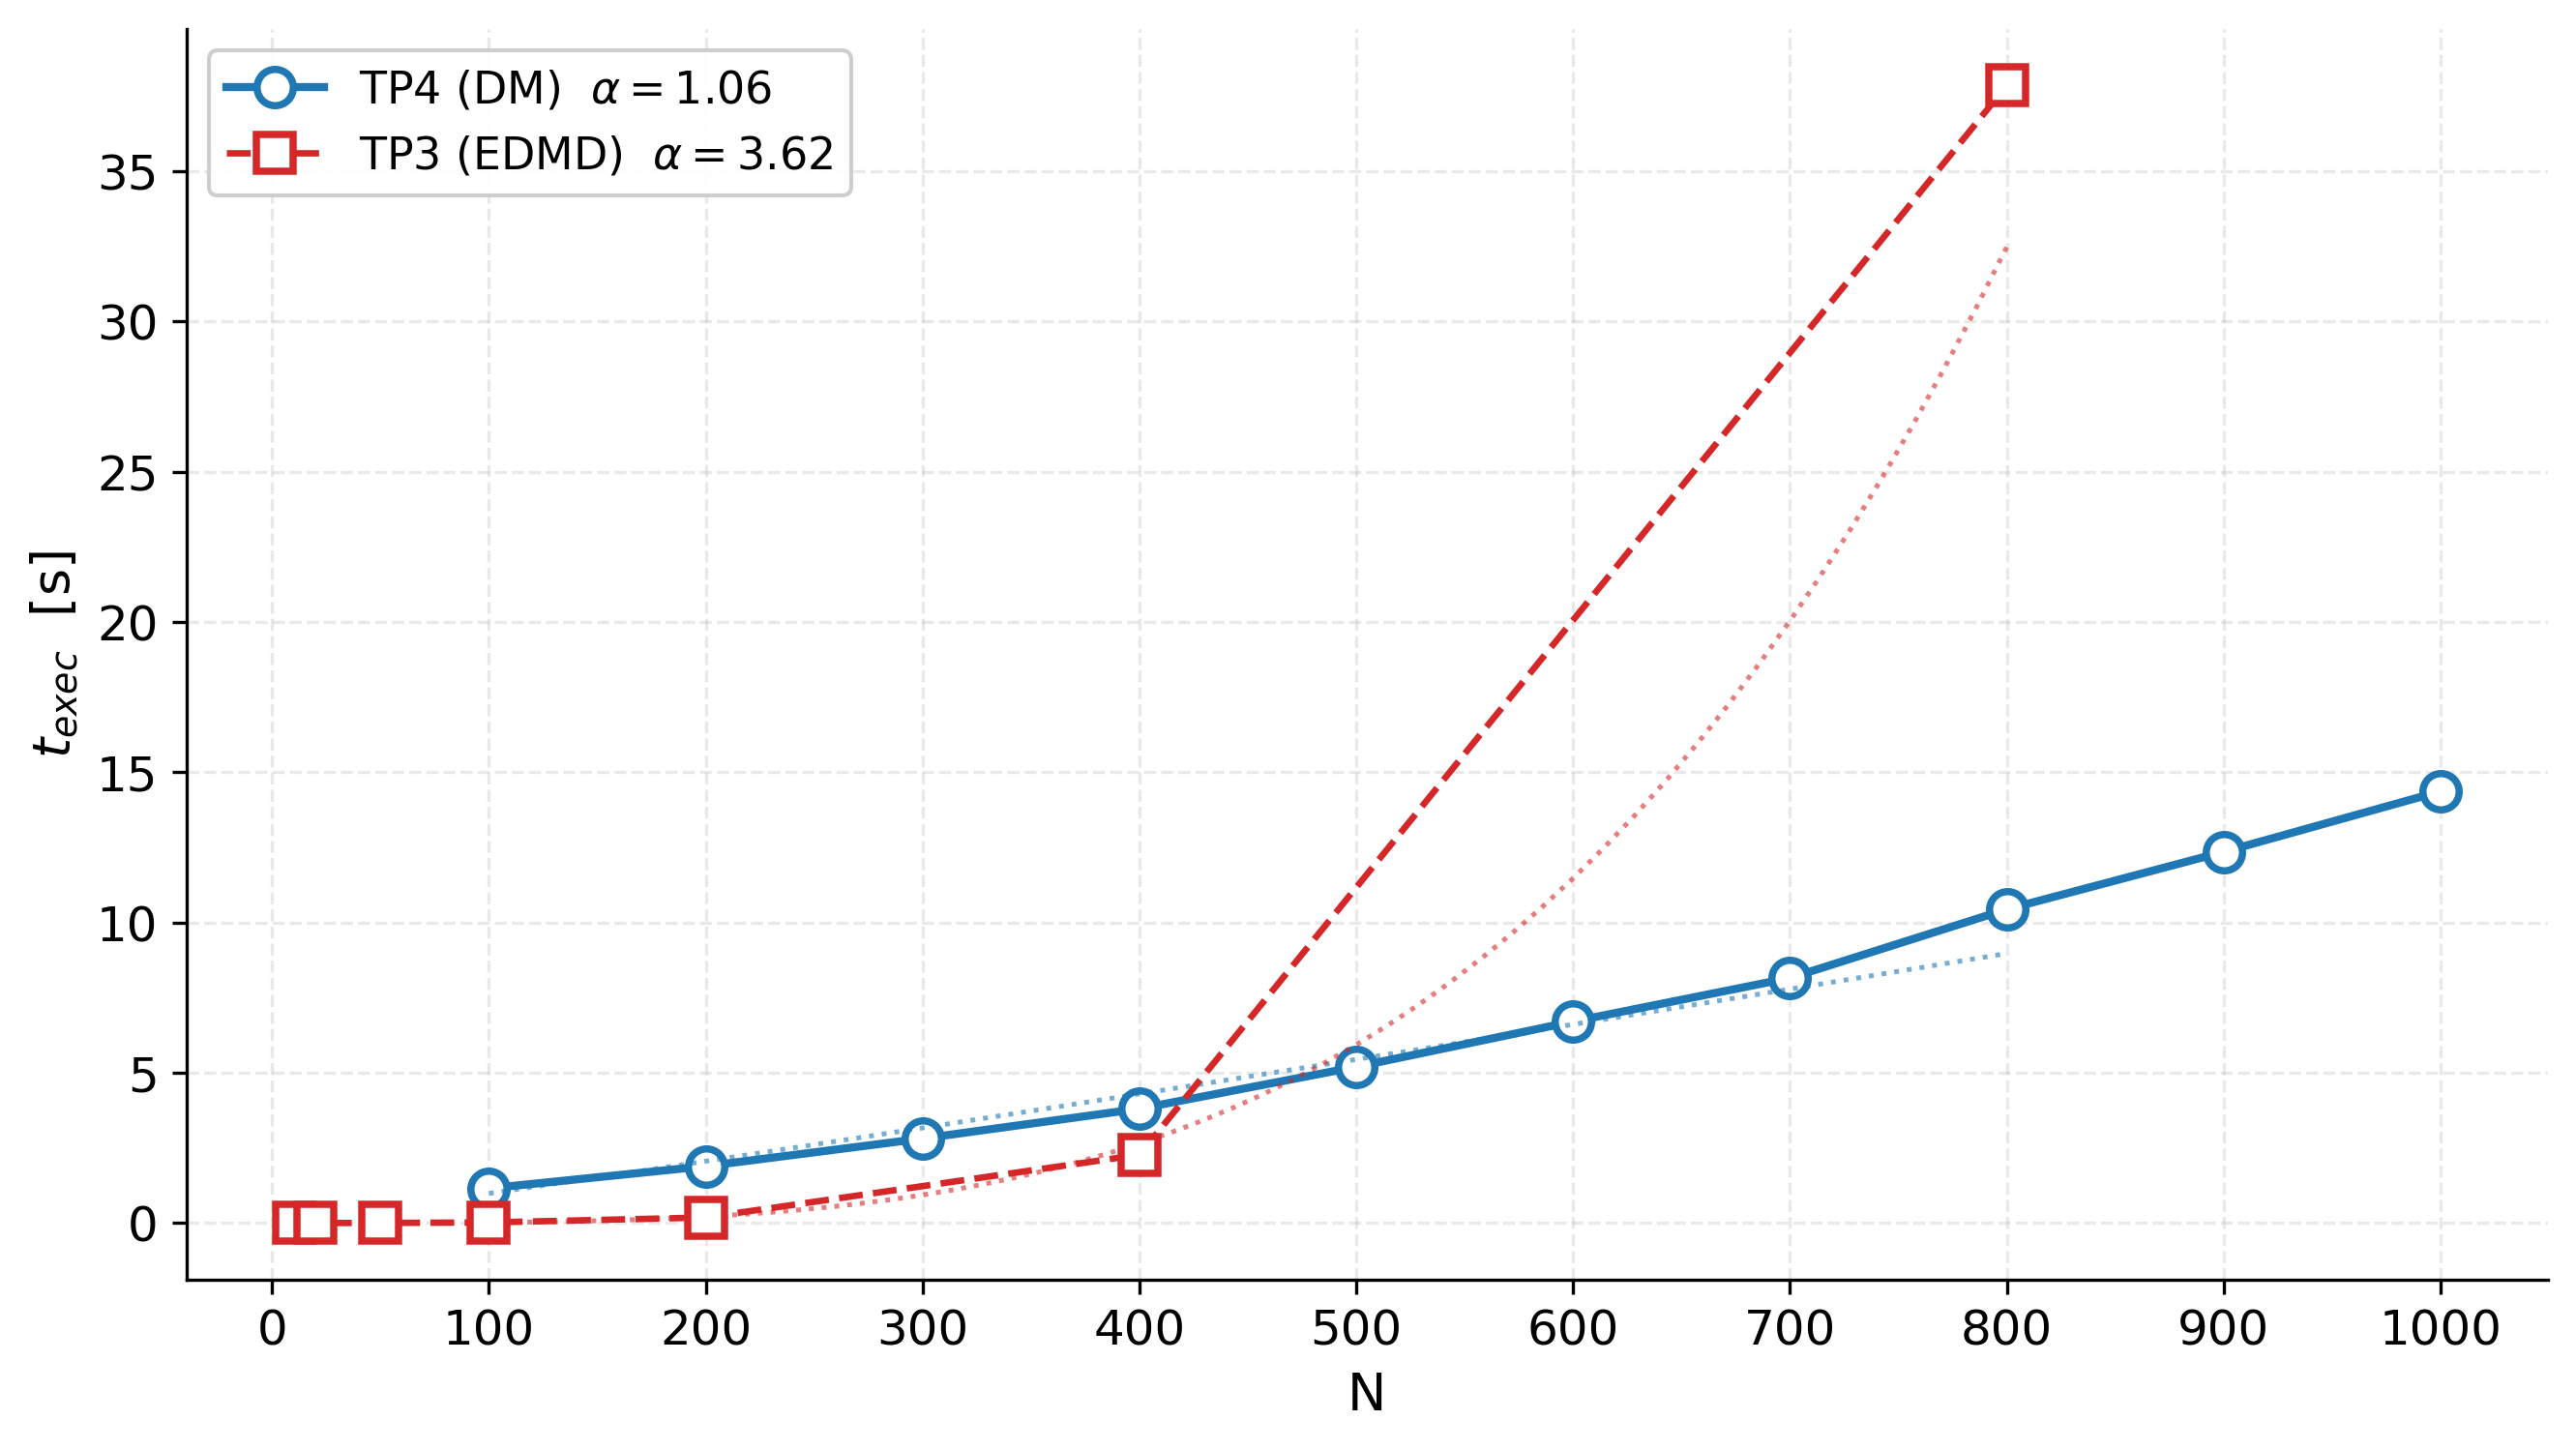
\includegraphics[width=\linewidth,height=0.70\textheight,keepaspectratio]{figures/04_s2_timing.png}
        \end{column}
        \begin{column}{0.32\textwidth}
            \textbf{Condiciones}
            \begin{itemize}\setlength\itemsep{1pt}
                \item $t_f = \SI{500}{s}$
                \item $k = 10^{3}$ \si{N/m}
                \item 1 realización por $N$
            \end{itemize}
            \vspace{0.2cm}
            \textbf{Observación}
            \begin{itemize}\setlength\itemsep{1pt}
                \item Log-log: ley de potencia $t_{\text{exec}} \propto N^{\alpha}$.
                \item DM time-driven vs.\ EDMD del TP3.
            \end{itemize}
        \end{column}
    \end{columns}
\end{frame}

% =============================================================================
% 1.2 Cfc y J(N)
% =============================================================================
\begin{frame}{Evolución temporal de $C_{fc}(t)$}
    \begin{columns}[T]
        \begin{column}{0.68\textwidth}
            \centering
            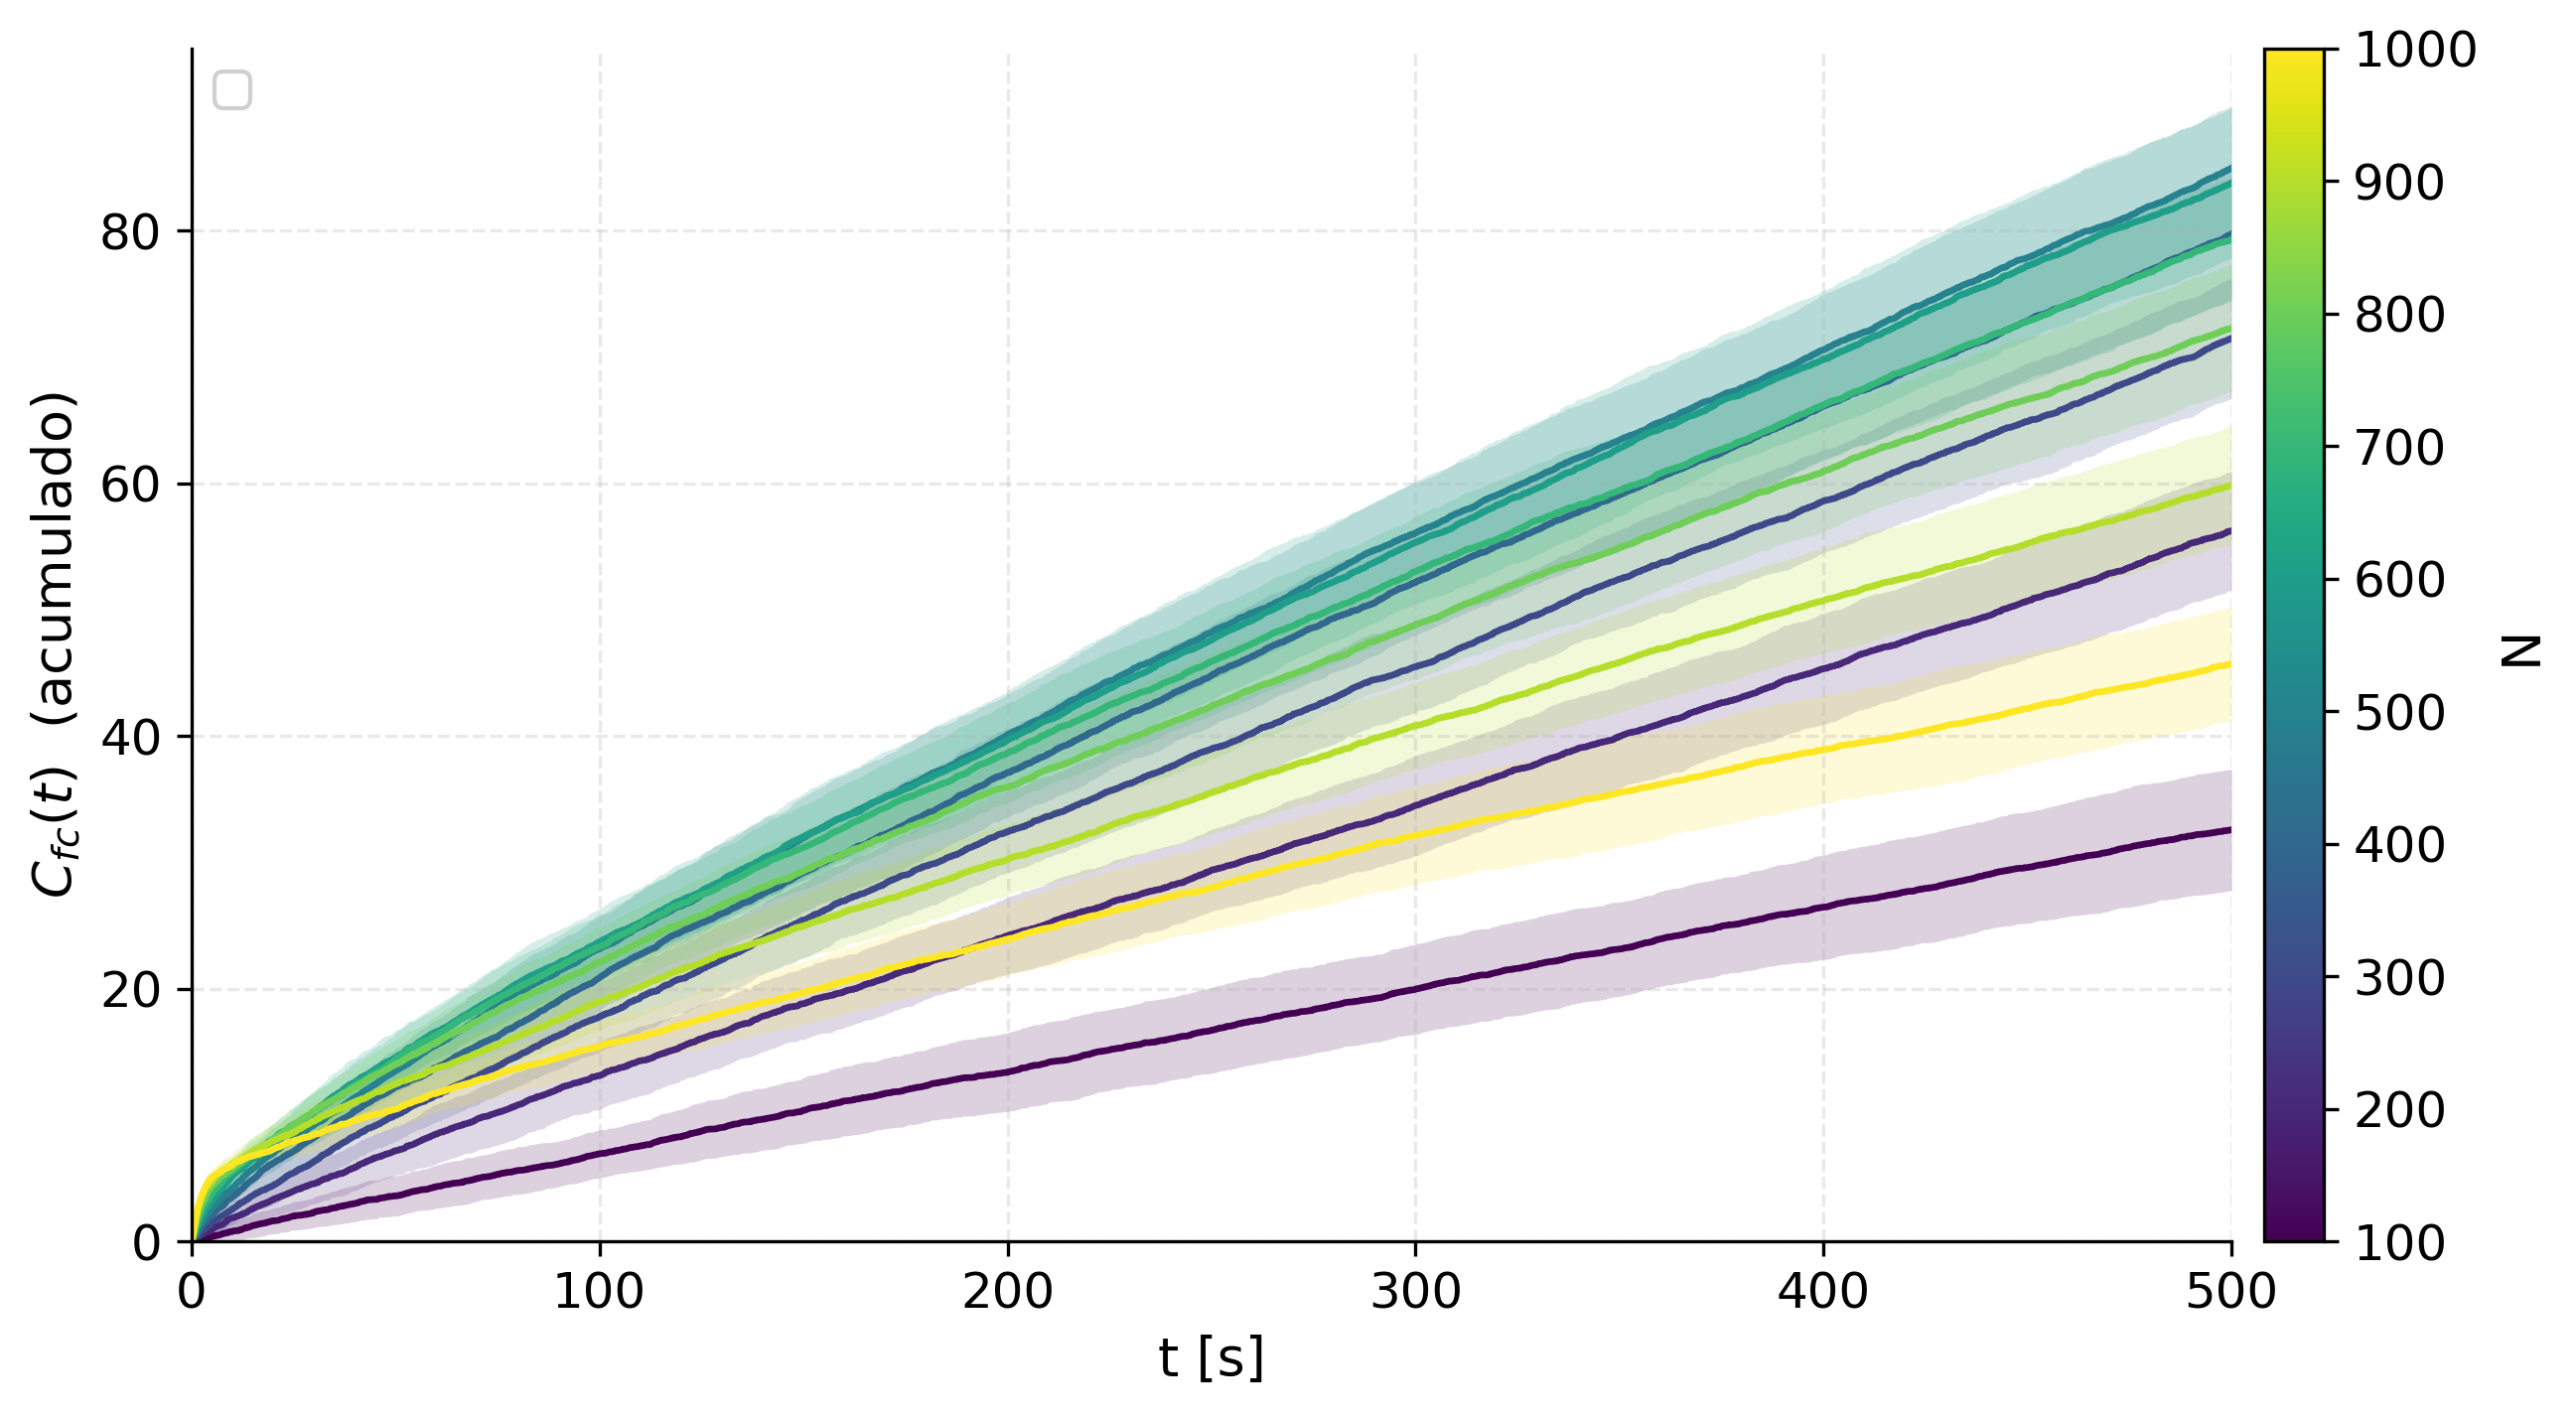
\includegraphics[width=\linewidth,height=0.70\textheight,keepaspectratio]{figures/05_s2_cfc_t.png}
        \end{column}
        \begin{column}{0.32\textwidth}
            \textbf{Observación}
            \begin{itemize}\setlength\itemsep{1pt}
                \item Régimen estacionario desde $t \approx 0$.
            \end{itemize}
        \end{column}
    \end{columns}
\end{frame}

\begin{frame}{Scanning rate $\langle J\rangle$ vs.\ $N$}
    \begin{columns}[T]
        \begin{column}{0.68\textwidth}
            \centering
            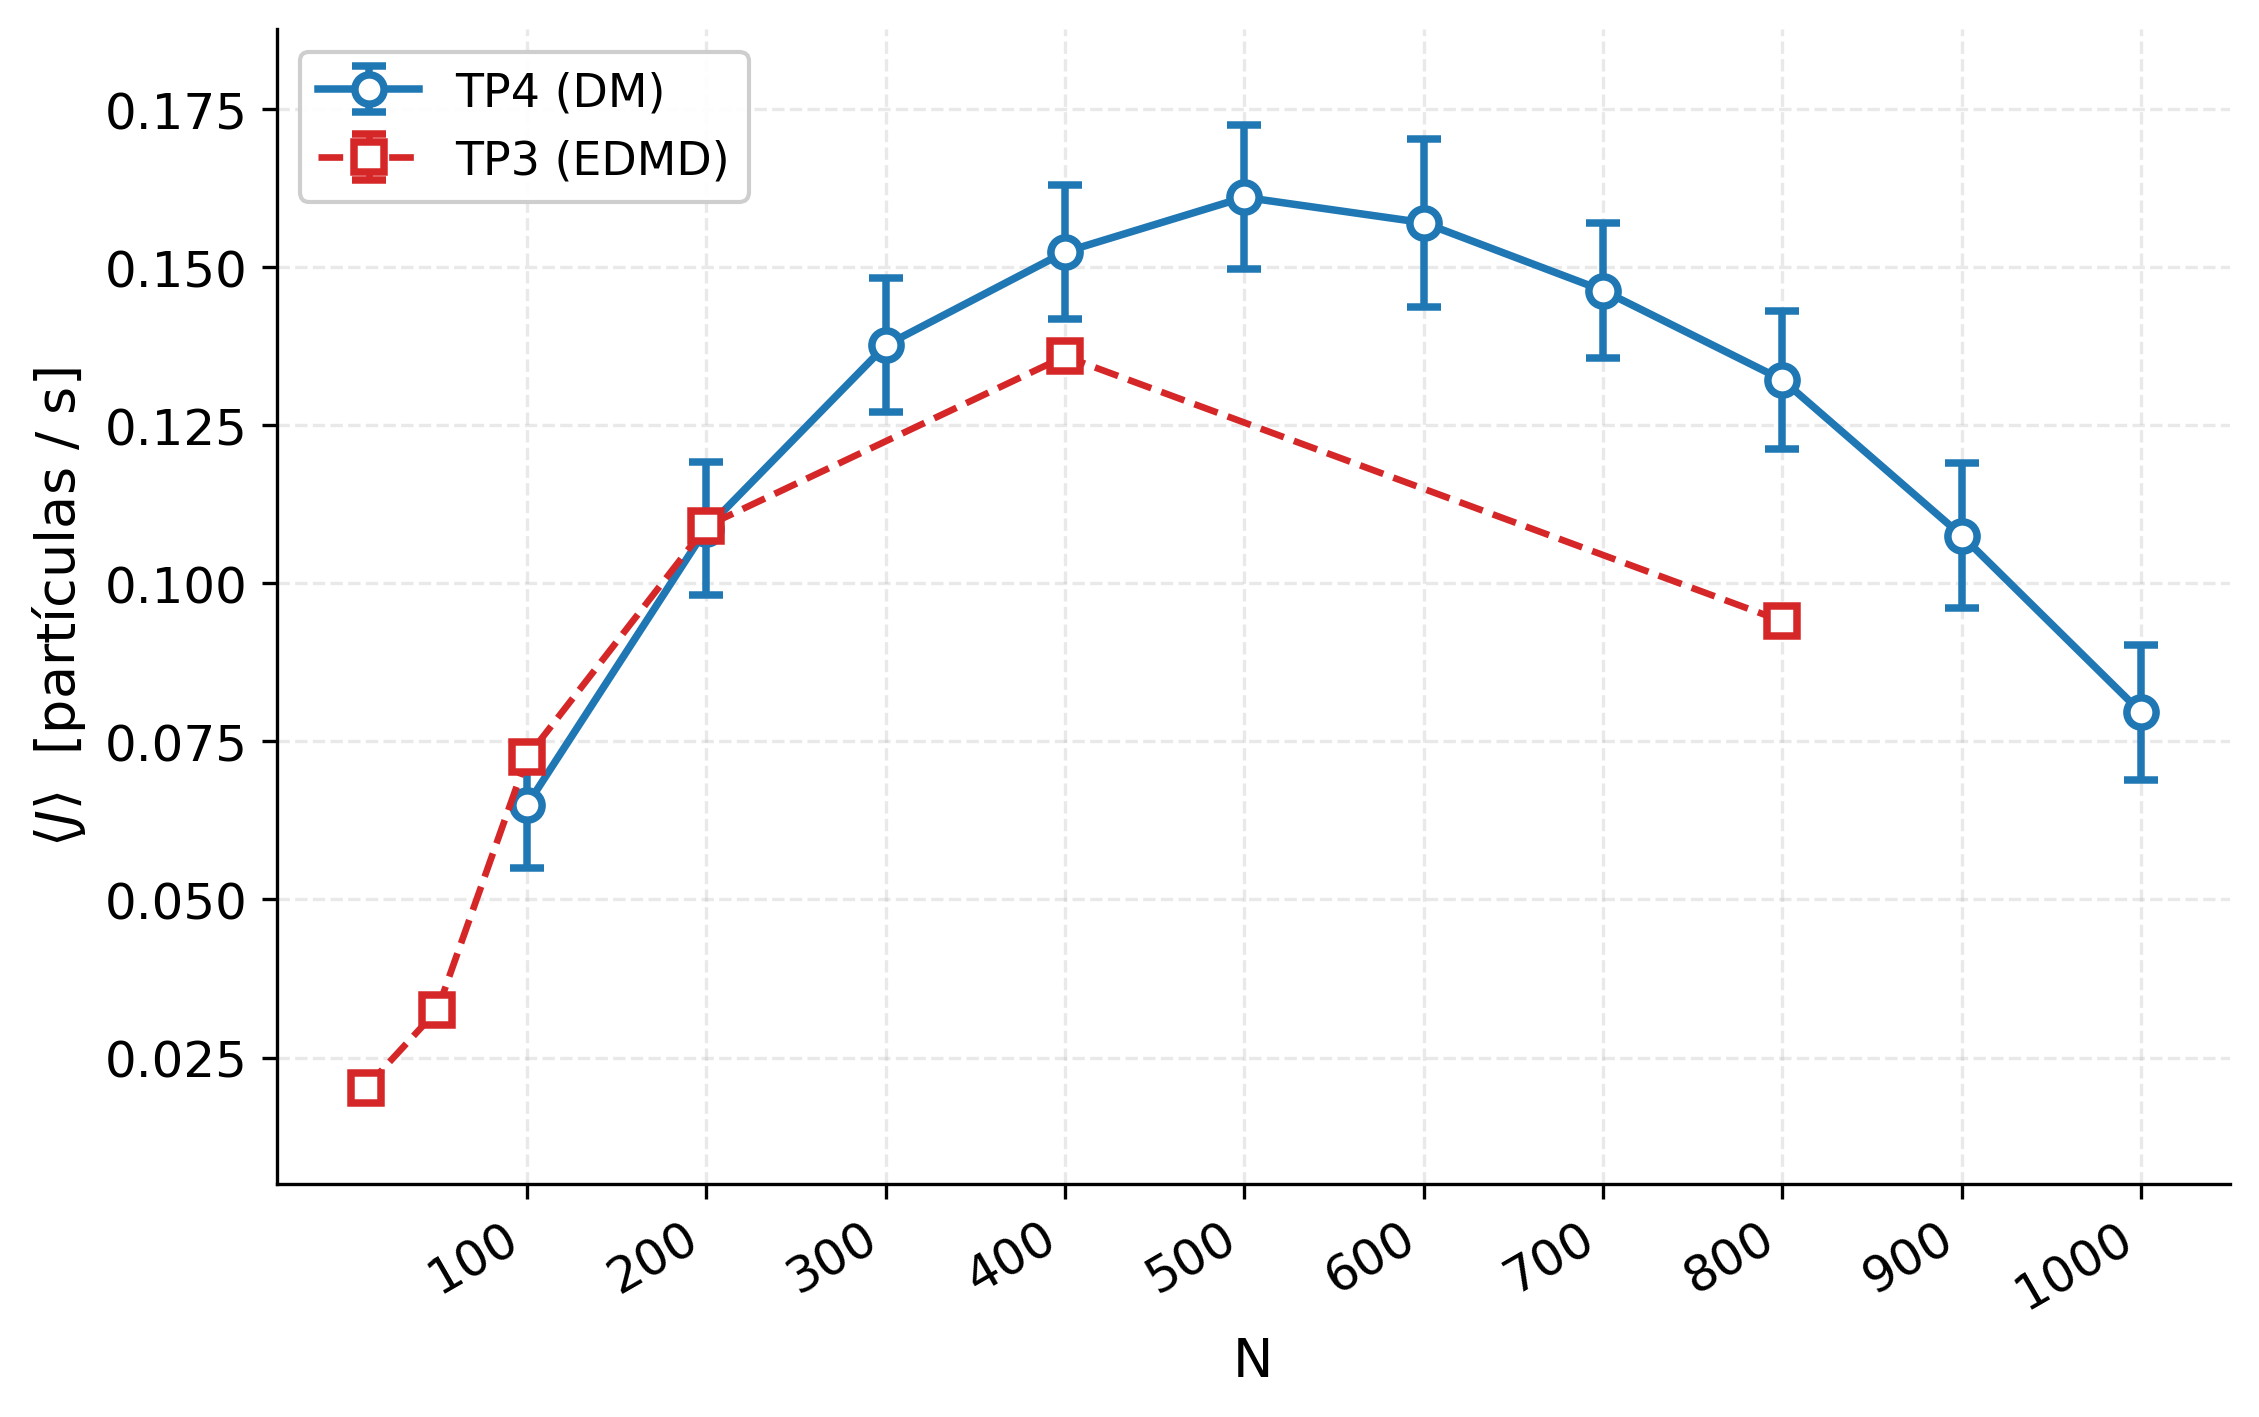
\includegraphics[width=\linewidth,height=0.70\textheight,keepaspectratio]{figures/06_s2_j_vs_n.png}
        \end{column}
        \begin{column}{0.32\textwidth}
            \textbf{Parámetros}
            \begin{itemize}\setlength\itemsep{1pt}
                \item $k = 10^{3}$ \si{N/m}
                \item $M = 100$ realizaciones
                \item Barras: $\sigma$ sobre realizaciones
            \end{itemize}
            \vspace{0.2cm}
            \textbf{Observación}
            \begin{itemize}\setlength\itemsep{1pt}
                \item Crece y satura con $N$.
                \item Máximo en $N \approx 500$.
                \item Similar a $J(N)$ del TP3.
            \end{itemize}
        \end{column}
    \end{columns}
\end{frame}

% =============================================================================
% 1.3 Perfiles radiales (como está)
% =============================================================================
\begin{frame}{Perfiles radiales -- $J_{\text{in}}(S)$}
    \begin{center}
        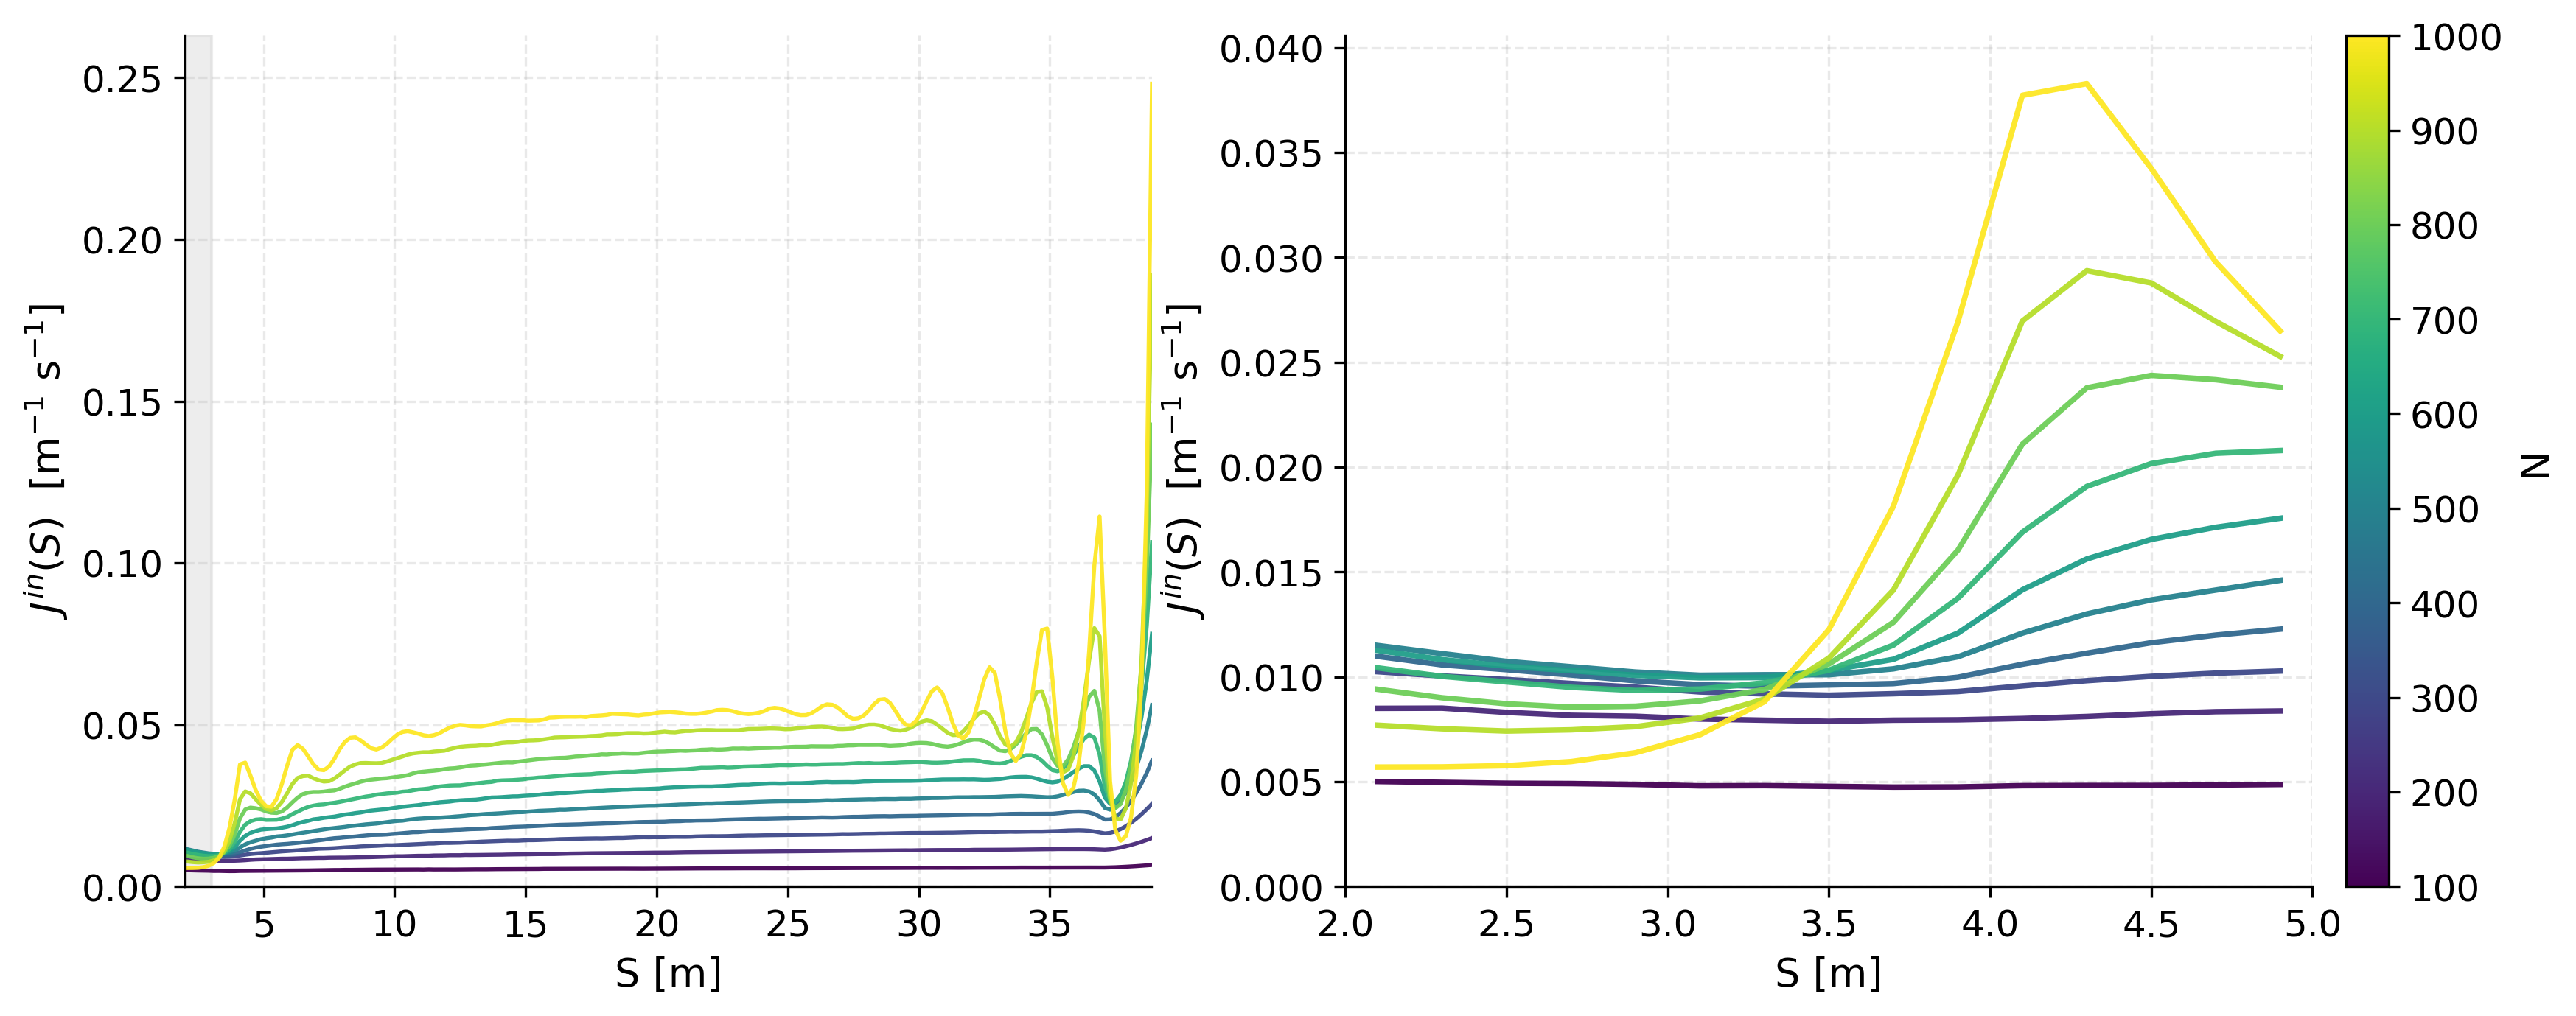
\includegraphics[width=0.92\linewidth,height=0.74\textheight,keepaspectratio]{figures/07_s2_radial.png}
    \end{center}
    {\footnotesize $k = 10^3$ N/m \quad $M = 100$ realizaciones \quad ventana $t \in [t_f/2,\,t_f]$ \quad capas $\mathrm{d}S = \SI{0.2}{m}$}
\end{frame}

\begin{frame}{Observables radiales cerca del obstáculo vs.\ $N$}
    \centering
    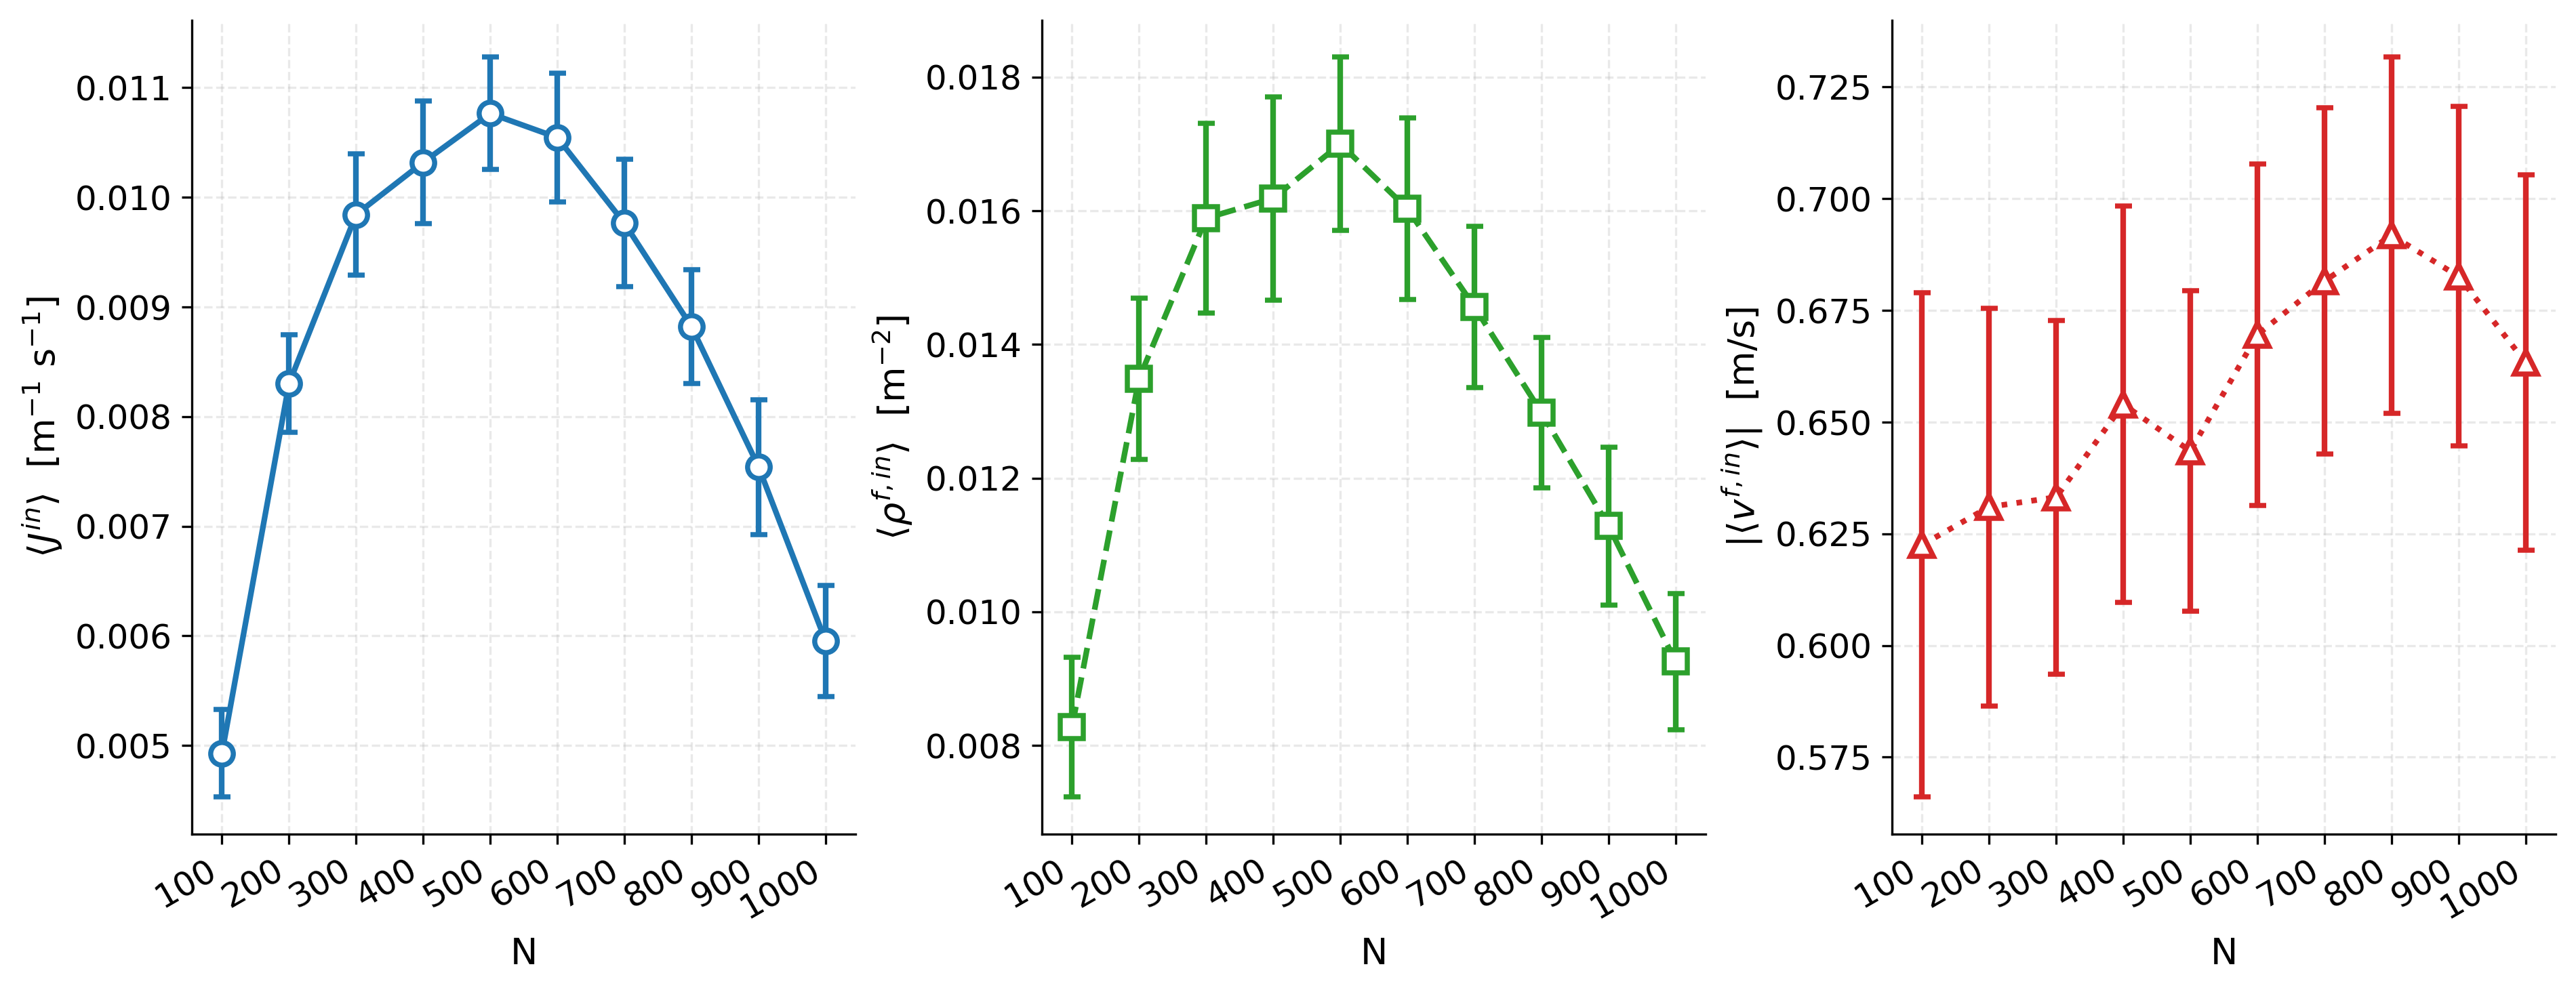
\includegraphics[width=0.92\linewidth,height=0.74\textheight,keepaspectratio]{figures/08_s2_radial_near.png}

    {\footnotesize Capa cercana al obstáculo $S \in [1.5,\,3.0]$ m, ponderado por $n_{\text{samples}}$. $k = 10^3$ N/m, $M = 100$ realizaciones.}
\end{frame}

% =============================================================================
% ANIMACIONES variando k (N fijo)
% =============================================================================
\begin{frame}{Animación -- $k = 10^{2}$ \si{N/m}, $N = 800$}
    \begin{columns}[T]
        \begin{column}{0.68\textwidth}
            \centering
            \videoorplaceholder{figures/k=100}{videos/k=100}%
                {Renderizar con \texttt{FrameExporter} (\texttt{Main2 --experiment animate
                --k 100 --N <N>}) y \texttt{scripts/render\_animations.sh}.
                Elegir $N$ representativo; ver \texttt{PLANPPT.md}.}
        \end{column}
        \begin{column}{0.32\textwidth}
            \textbf{Condiciones}
            \begin{itemize}
                \item $k = 10^{2}$ \si{N/m}
                \item $N = 800$
                \item $\Delta t = \SI{5e-3}{s}$
            \end{itemize}
        \end{column}
    \end{columns}
\end{frame}

\begin{frame}{Animación -- $k = 10^{4}$ \si{N/m}, $N = 800$}
    \begin{columns}[T]
        \begin{column}{0.68\textwidth}
            \centering
            \videoorplaceholder{figures/k=10000}{videos/k=10000}%
                {Renderizar con \texttt{FrameExporter} (\texttt{Main2 --experiment animate
                --k 10000 --N <N>}) y \texttt{scripts/render\_animations.sh}.
                Mismo $N$ que la slide anterior para comparar.}
        \end{column}
        \begin{column}{0.32\textwidth}
            \textbf{Condiciones}
            \begin{itemize}
                \item $k = 10^{4}$ \si{N/m}
                \item $N = 800$
                \item $\Delta t = \SI{1e-3}{s}$
            \end{itemize}
        \end{column}
    \end{columns}
\end{frame}

% =============================================================================
% 1.4 Variación de k
% =============================================================================
\begin{frame}{$\Delta t$ elegido por $k$}
    \centering
    \vspace{0.3cm}
    \begin{tabular}{c c c}
        \hline
        $k$ \si{[N/m]} & $\Delta t$ elegido \\
        \hline
        $10^{1}$  & $\approx \SI{1e-2}{s}$ \\
        $10^{2}$  & $\approx \SI{5e-3}{s}$ \\
        $10^{3}$  & $\approx \SI{1e-3}{s}$ \\
        $10^{4}$  & $\approx \SI{1e-3}{s}$ \\
        $10^{5}$  & $\approx \SI{5e-4}{s}$ \\
        \hline
    \end{tabular}

    \vspace{0.5cm}
    \begin{itemize}\setlength\itemsep{2pt}
        \item Mismo estudio que para $k = 10^{3}$: evolución de $\Delta E_{\text{tot}}/E_0$ vs.\ $t$ por $\Delta t$,
              pendiente $S_e$ vs.\ $\Delta t$.
    \end{itemize}
\end{frame}

\begin{frame}{Scanning rate $\langle J\rangle$ y flujo $\langle J_{\text{in}}|_{S\sim 2}\rangle$ vs.\ $N$ -- barrido en $k$}
    \begin{center}
        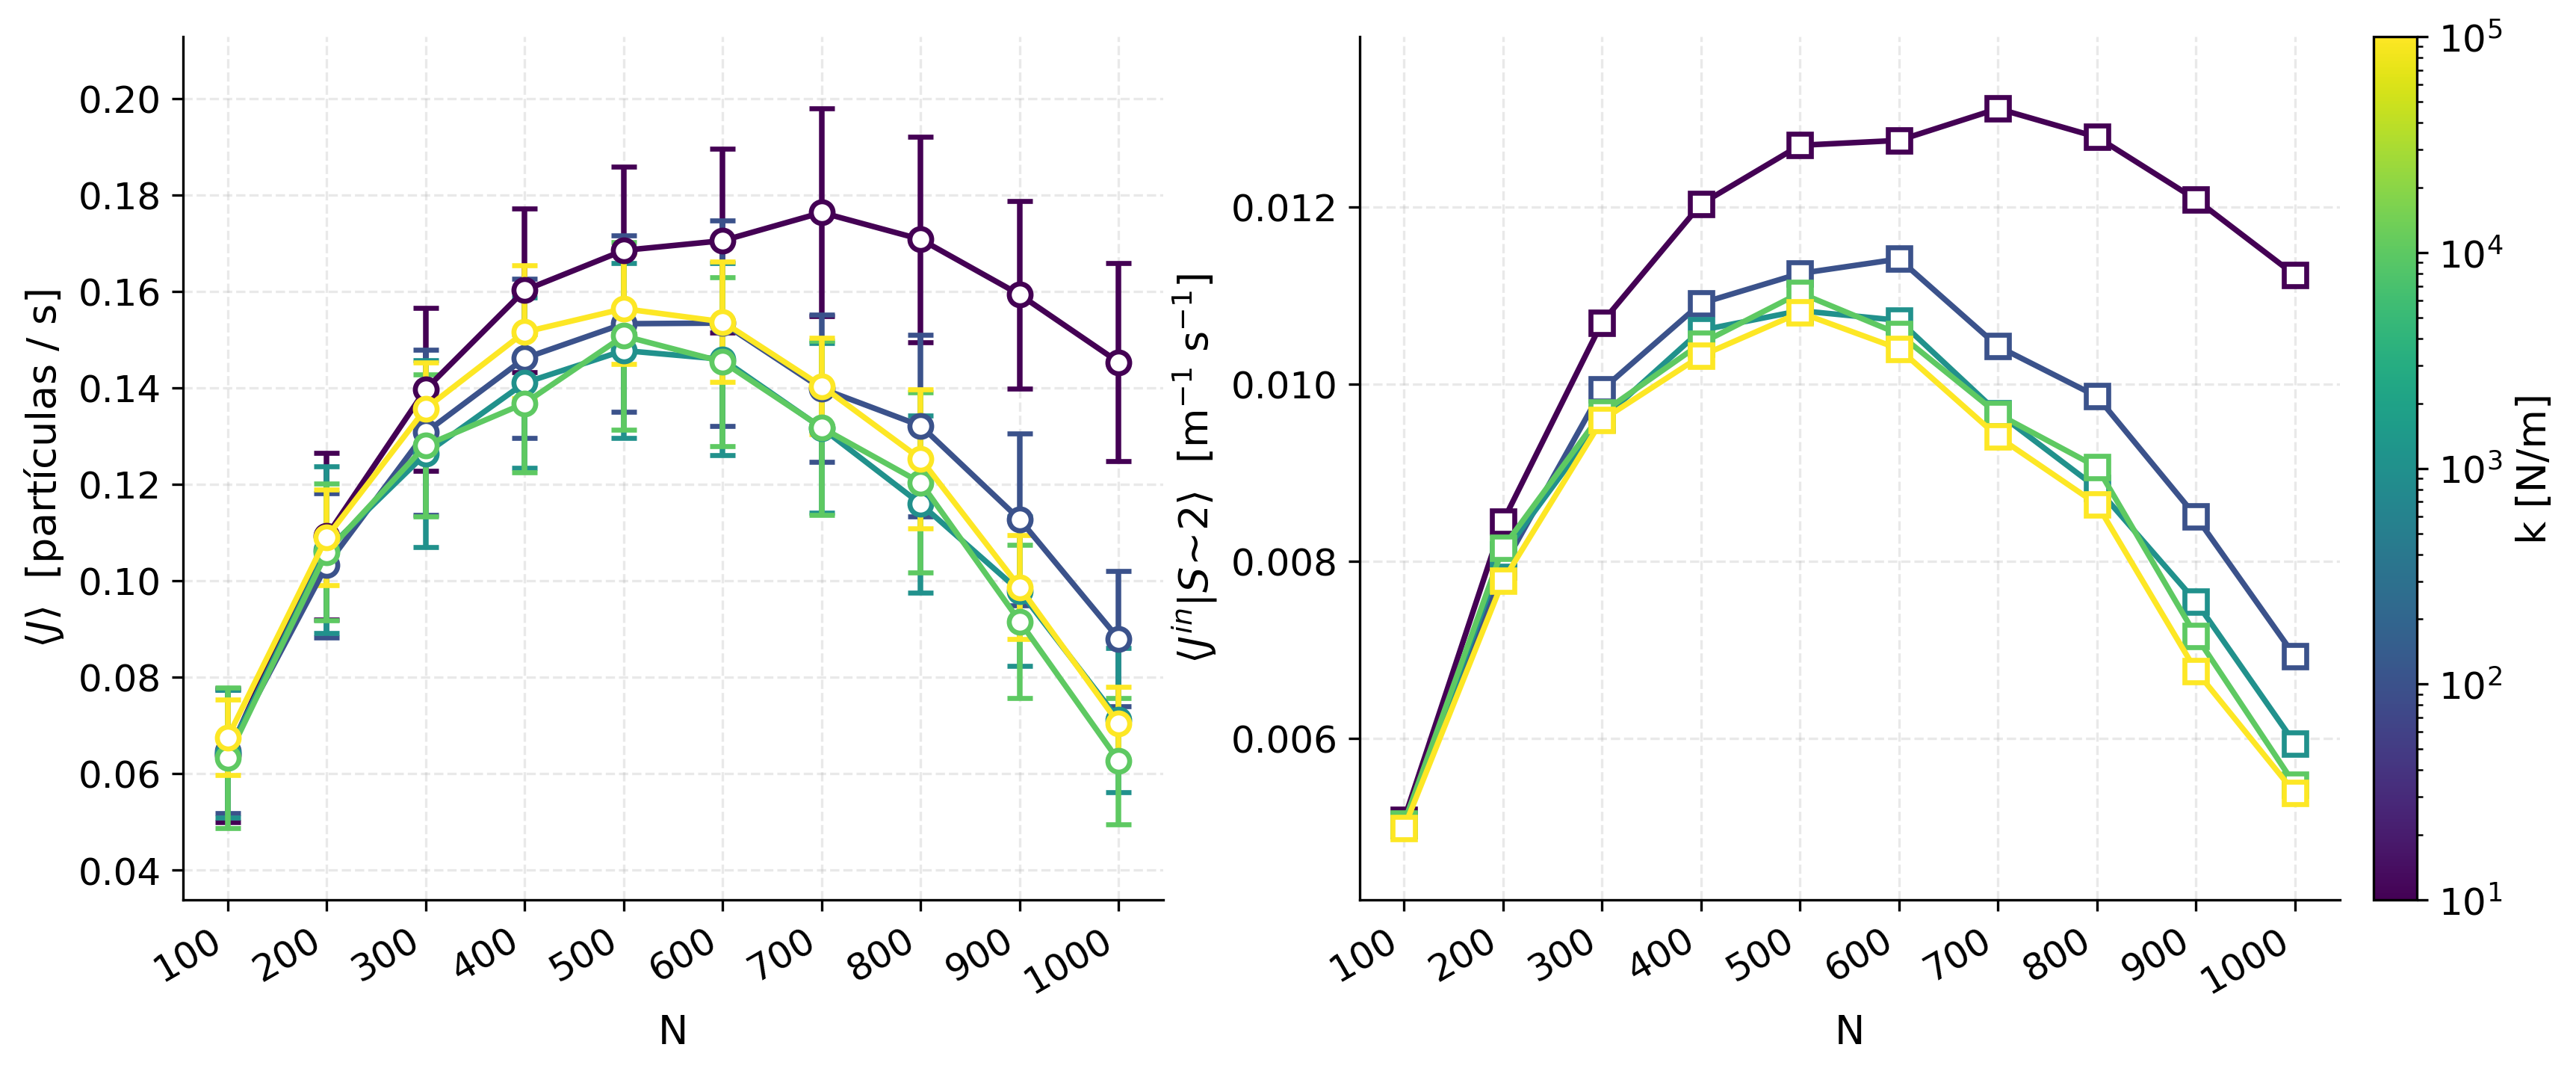
\includegraphics[width=0.96\linewidth,height=0.78\textheight,keepaspectratio]{figures/09_s2_k_sweep.png}
    \end{center}
\end{frame}

\begin{frame}{Escalar característico vs.\ $k$ para $N$ fijo}
    \begin{columns}[T]
        \begin{column}{0.68\textwidth}
            \centering
            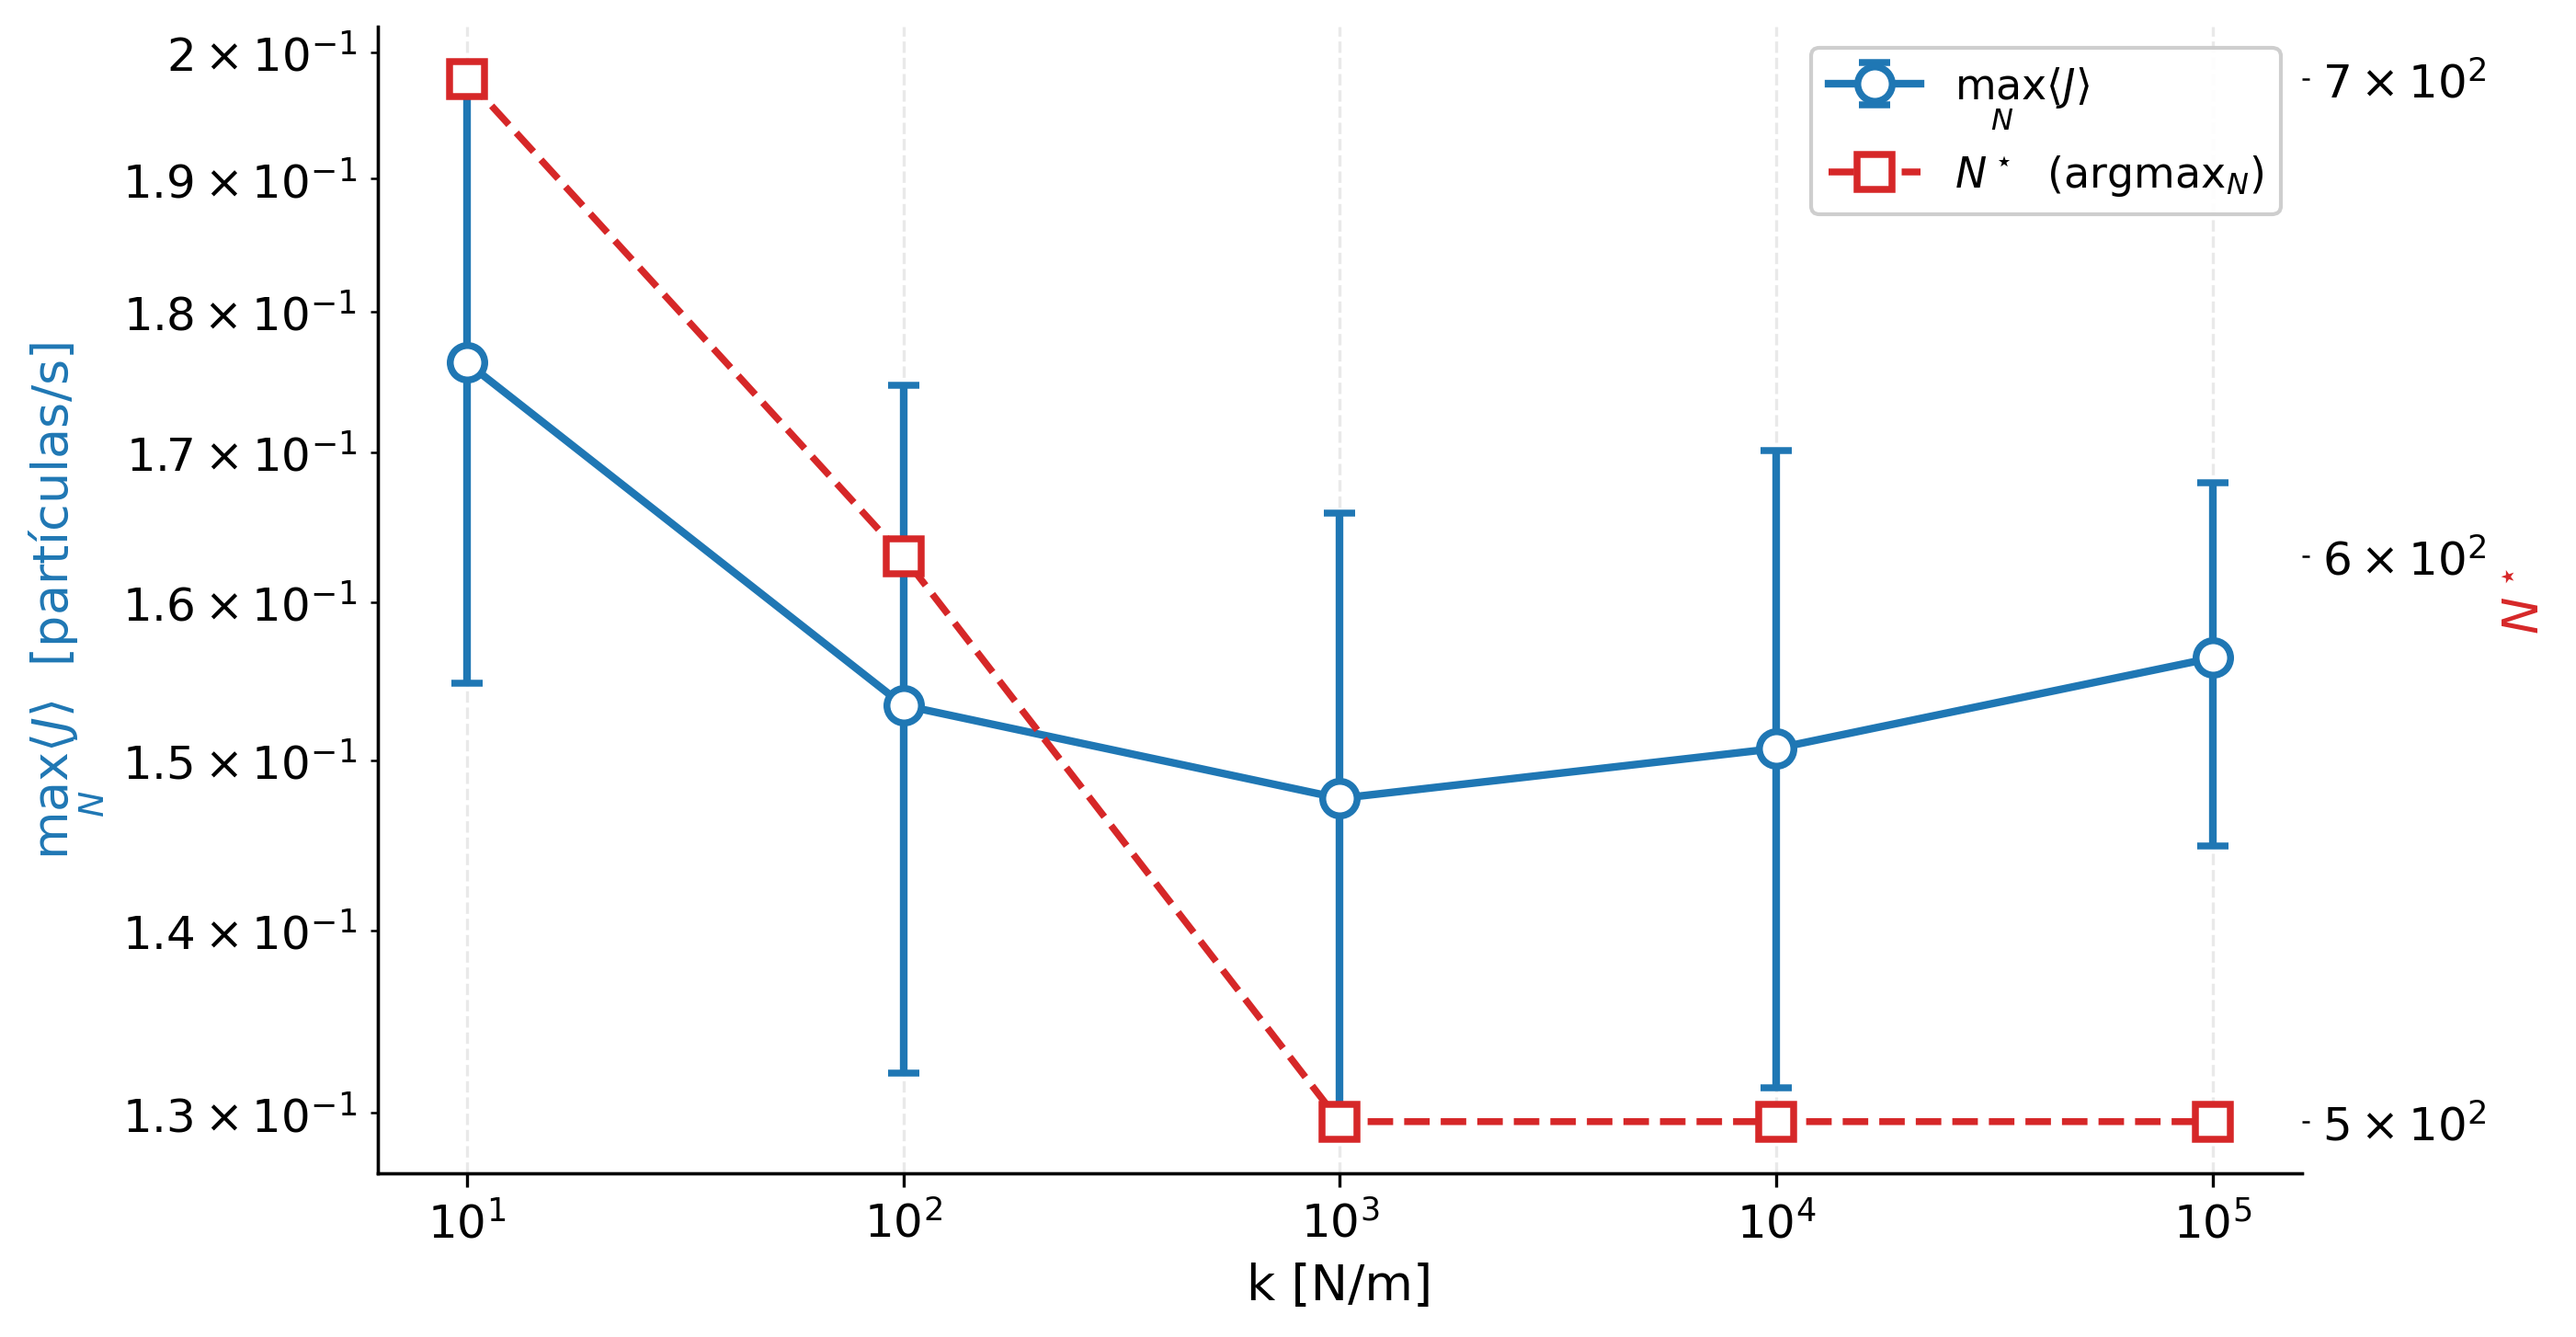
\includegraphics[width=\linewidth,height=0.70\textheight,keepaspectratio]{figures/10_s2_k_scalar.png}
        \end{column}
        \begin{column}{0.32\textwidth}
            \textbf{Escalar}: $\max_N \langle J\rangle(k)$
            \vspace{0.2cm}
            \begin{itemize}\setlength\itemsep{2pt}
                \item $\max_N \langle J\rangle$ constante para todo $k$.
            \end{itemize}
        \end{column}
    \end{columns}
\end{frame}

% =============================================================================
% CONCLUSIONES
% =============================================================================
\section{Conclusiones}

\begin{frame}[plain,c]
    \centering
    {\usebeamercolor[fg]{structure}\fontsize{48}{56}\selectfont Conclusiones\par}
\end{frame}

\begin{frame}{Conclusiones}
    \begin{itemize}\setlength\itemsep{4pt}
        \item \textbf{Sistema 1}: Gear-5 con $\alpha_0 = 3/16$ minimiza el ECM en todo el rango de $\Delta t$ estudiado; pendientes en log-log consistentes con el orden teórico de cada integrador.
        \item \textbf{Sistema 2}: el scanning rate $\langle J\rangle$ crece con $N$ y satura; el régimen cerca del obstáculo está dominado por la densidad de partículas frescas entrantes.
        \item La fuerza elástica blanda con $k$ creciente reproduce el límite event-driven del TP3.
        \item DM time-driven escala mejor con $N$ que EDMD en el rango estudiado.
    \end{itemize}
\end{frame}

% =============================================================================
% CIERRE
% =============================================================================
{
    \setbeamertemplate{footline}{}
    \begin{frame}[plain,c]
        \centering
        {\fontsize{48}{56}\selectfont Muchas gracias\par}
    \end{frame}
}

\end{document}
